\documentclass[a4paper,14pt]{extreport}
\usepackage[utf8]{inputenc}
\usepackage[english,russian]{babel}
% \usepackage[dvips]{graphicx}
\usepackage[pdftex]{graphicx}
\usepackage{geometry}
\geometry{left=25mm}
\geometry{right=20mm}
\geometry{top=20mm}
\geometry{bottom=20mm}
\graphicspath{{image/}}
\usepackage[usenames]{color}
\usepackage{colortbl}
\usepackage{multirow}
\usepackage{amssymb,amsfonts,amsmath,mathtext,cite,enumerate,float}
\usepackage{setspace}
\usepackage{indentfirst}
\onehalfspacing


\begin{document}
\begin{titlepage}
\begin{table}[]
    \centering
    \begin{tabular}{rcl}
    Автономная некоммерческая &
    \multirow{4}{*}{
\includegraphics[width=40mm]{image/logo.eps}}
          & Autonomous noncommercial \\
    организация высшего  & & organization of higher \\
    образования & & education \\
    «Университет Иннополис»  &
     & «Innopolis University» \\
    \hline
    \hline
    \end{tabular}
    \label{tab:my_label}
\end{table}
\vline
\vspace{20mm}

\begin{center}
\textbf{АННОТАЦИЯ \\ НА ВЫПУСКНУЮ КВАЛИФИКАЦИОННУЮ РАБОТУ  \\
ПО НАПРАВЛЕНИЮ ПОДГОТОВКИ \\ 09.03.01 --- «ИНФОРМАТИКА И ВЫЧИСЛИТЕЛЬНАЯ ТЕХНИКА»}
\end{center}
\vspace{20mm}


    \begin{tabular}{ll
|>{\columncolor[gray]{.9}}l|}
\cline{3-3}
\textbf{Тема:} &
     &
    \makebox[133mm][l]{Альтернативы статической типизации для Clojure}    \\
    &&\\
    && \\
    &&  \\
\cline{3-3}
    \end{tabular}
\vspace{5mm}


    \begin{tabular}{ll
|>{\columncolor[gray]{.9}}l|l
|>{\columncolor[gray]{.9}}l|}
\cline{3-3} \cline{5-5}
Выполнил &
     &
    \makebox[77mm][l]{Тропин Андрей Геннадьевич}   &
    &    \\
    &&&&
    \makebox[39.5mm]{\textcolor[gray]{.7}{подпись}} \\
    &&&& \\
    \cline{3-3} \cline{5-5}
    \end{tabular}
\vspace{5mm}

\vspace{\fill}

\begin{center}
Иннополис, 2017
\end{center}
\end{titlepage}


\newpage
% \noindent {\large \textbf{Содержание}} \\

\chapter*{Содержание}
\documentclass[a4paper,14pt]{report}
\usepackage[T2A]{fontenc}
\usepackage[utf8]{inputenc}
\usepackage[russian,english]{babel}
% \usepackage[dvips]{graphicx}
\usepackage[pdftex]{graphicx}
\usepackage{geometry}
\geometry{left=25mm}
\geometry{right=20mm}
\geometry{top=20mm}
\geometry{bottom=20mm}
\graphicspath{{figures/}}
\usepackage[usenames]{color}
\usepackage{colortbl}
\usepackage{multirow}
% \usepackage{setspace}
% \onehalfspacing

\usepackage{thesis}
\usepackage{minted}

\begin{document}

\pagenumbering{roman}

\begin{titlepage}
\begin{table}[]
    \centering
    \begin{tabular}{rcl}
    Автономная некоммерческая &
    \multirow{4}{*}{
\includegraphics[width=40mm]{figures/logo.eps}}
    & Autonomous noncommercial \\
    организация высшего  & & organization of higher \\
    образования & & education \\
    «Университет Иннополис»  &
     & «Innopolis University» \\
    \hline
    \hline
    \end{tabular}
    \label{tab:my_label}
\end{table}
\vline
\vspace{0mm}

\begin{center}
\textbf{
ВЫПУСКНАЯ КВАЛИФИКАЦИОННАЯ РАБОТА  \\
ПО НАПРАВЛЕНИЮ ПОДГОТОВКИ \\
09.03.01 --- «ИНФОРМАТИКА И ВЫЧИСЛИТЕЛЬНАЯ ТЕХНИКА»}
\vspace{5mm}

\textbf{GRADUATE THESIS    \\
MAJOR: "COMPUTER SCIENCE"}
\end{center}
\vspace{20mm}


    \begin{tabular}{ll
|>{\columncolor[gray]{.8}}l|}
\cline{3-3}
\textbf{Тема:} &
    \makebox[0.5mm] &
                      \makebox[135mm][l]{Альтернативы статической типизации для Clojure}    \\
    &&\\
\cline{3-3}
    \end{tabular}
\vspace{5mm}

    \begin{tabular}{ll
|>{\columncolor[gray]{.8}}l|}
\cline{3-3}
\textbf{Topic:} &
     &
       \makebox[135mm][l]{Alternatives of static type system for Clojure}    \\
    &&\\
\cline{3-3}
    \end{tabular}
\vspace{5mm}


    \begin{tabular}{ll
|>{\columncolor[gray]{.8}}l|l
|>{\columncolor[gray]{.8}}l|}
\cline{3-3} \cline{5-5}
Работу выполнил / &
    \makebox[0.5mm] &
    \makebox[64mm][l]{Тропин Андрей Геннадьевич/}  &
    &       \\
Thesis is executed by  &
    \makebox[0.5mm] &
    \makebox[64mm][l]{Tropin Andrei Gennadievich}  &
    &
    \makebox[40mm]{\textcolor[gray]{.6}{подпись / signature}}     \\
    % &&&&&
\cline{3-3} \cline{5-5}  \\
    \end{tabular}
\vspace{5mm}

    \begin{tabular}{ll
|>{\columncolor[gray]{.8}}l|l
|>{\columncolor[gray]{.8}}l|}
\cline{3-3} \cline{5-5}
Научный руководитель / &
     &
    \makebox[57mm][l]{Мануэль Маццара /}  &
    &       \\
Thesis supervisor  &
     &
    \makebox[57mm][l]{Manuel Mazzara}  &
    &
    \makebox[40mm]{\textcolor[gray]{.6}{подпись / signature}}     \\
    % &&&&&
\cline{3-3} \cline{5-5}  \\
    \end{tabular}
\vspace{\fill}

\begin{center}
Иннополис, Innopolis, 2017
\end{center}
\end{titlepage}

\addcontentsline{toc}{chapter}{Abstract}
\begin{center}
\textbf{\large Abstract}
\end{center}

This document provides information on how to workaround some drawbacks of
dynamically typed languages. Lack of documentation about function parameters
types. The need to write a lot of tests to check consistency of the project and
integration between components. Implementation hardly rely on
\textbf{clojure.spec} library.

First paragraph: state what the thesis is about, give a simple statement of aims and
methods

Second paragraph: explain the structure of the thesis and say something about the
content

Third paragraph: give a concluding statement, including a short summary of the
results

Additional information about writing abstract can be found here: \\
% https://www.th-wildau.de/fileadmin/dokumente/studiengaenge/europaeisches_management/dokumente/Dokumente_EM_Ba/Abstracts_in_English.pdf

\vspace{1cm}

% \emph{``The purpose of the abstract, which should not exceed 150 words for
% a Masters' thesis or 350 words for a Doctoral thesis, is to provide
% sufficient information to allow potential readers to decide on relevance
% of the thesis. Abstracts listed in Dissertation Abstracts International
% or Masters' Abstracts International should contain appropriate key
% words and phrases designed to assist electronic searches.''}

\hfill --- MUN School of Graduate Studies

\addcontentsline{toc}{chapter}{Acknowledgements}
\begin{center}
\textbf{\large Acknowledgements}
\end{center}

Put your acknowledgements here...

\vspace{1cm}

\emph{``Intellectual and practical assistance, advice, encouragement and
sources of monetary support should be acknowledged. It is appropriate to
acknowledge the prior publication of any material included in the thesis
either in this section or in the introductory chapter of the thesis.''}

\hfill --- MUN School of Graduate Studies

\tableofcontents

\addcontentsline{toc}{chapter}{List of Tables}
\listoftables

\addcontentsline{toc}{chapter}{List of Figures}
\listoffigures


% Always make sure to tell a story in CS by using
% this order:
% 1)WHY
% 2)WHAT
% 3)HOW
\pagenumbering{arabic}
\chapter{Introduction}
\label{chap:intro}

\section{Overview}

There are two main approaches of type checking: static and dynamic. Advocates of
first approach say that benefits of static type checking include earlier
detection of bugs and mistakes (e.g. preventing adding string to an integer),
inline documentation and additional data for advanced code competition, useful
information for compiler, which helps to make optimizations (e.g. replacing
virtual calls by direct calls, when type of the caller are known), improved
runtime efficiency (e.g. not necessary to do dynamic dispatching).

On the other hand, there are also advocates of dynamic type checking who states
that languages with such approach have following advantages: interactive dynamic
development (e.g. REPL driven development + TDD, where tests can be rerun
without recompilation of the whole project), fast prototyping (e.g. type
decisions can be postponed, language are much more expressive and more suitable
for development of systems with rapidly changing or unknown requirements).

Static type checking is a good tool, but it necessary to understand that it
doesn't guarantee programs to be bug-free and correct because it provides
compile-time abstraction over run-time behavior of the software system this
means that some errors can be caught, but execution of the program can still go
wrong. Moreover static typing force to make decisions earlier, slowdown
compilation and make interactive development nearly impossible.

Nowadays many people/teams/companies interested in making data-intensive
systems, just take a look at current trends: data-driven approaches, BigData,
machine learning becomes more and more popular. The reason is clear: huge amount
of data allows to extract useful knowledge, but we need some tools to do it.
Probably dynamism is one of the most important thing for such kind of software
systems because majority of data is not fully structured, according to research
project report of Berkeley University \ref{lymanmuch} around 95\%. In cases when
structure is known up front after few steps people or algorithms generates
queries based on run-time information and data also gets dynamic nature.

Dynamic type checking is a good tool for data-intensive or other kind of dynamic
systems, but it also necessary to understand that it has some trade-offs. It is
much harder to refactor, develop and maintain systems with such type checking
because any even small change can break the system and nobody will know it until
fault will occur later in run-time. There are some techniques, which helps to
deal with it like Test-driven development \ref{beck2003test} or Contract-driven
development \ref{meyer2007contract}, but they doesn't solve all the problems.
Sometimes it is pretty handy to define shape of the date up front to check if
current data conform the specification or to generate data samples from such
specifications.

Information about when and what type checking better to use can be found in
\cite{meijer2004static}, it states that use static typing where possible and
dynamic when needed, but what if there is no possibility to choose type checking
system and it is necessary to use dynamically typed language? Can benefits of
static type checking be achieved in such environment?


\section{Goals of the project}

One of the first tasks of a researcher is defining the scope of a study, i.e., its area (theme, field) and the amount of information to be included. Narrowing the scope of your thesis can be time-consuming. Paradoxically, the more you limit the scope, the more interesting it becomes. This is because a narrower scope lets you clarify the problem and study it at greater depth, whereas very broad research questions only allow a superficial treatment.

The research question can be formulated as one main question with (a few) more specific sub-questions or in the form of a hypothesis that will be tested.

Your research question will be your guide as your writing proceeds. If you are working independently, you are also free to modify it as you go along.

How do you know that you have drafted a research question? Most importantly, a research question is something that can be answered. If not, you have probably come up with a theme or field, not a question.

Some tips:

% I will hire someone, who will explain problems of this thesis
Use interrogative words: how, why, which (factors/situations) etc.
Some questions are closed and only invoke concrete/limited answers. Others will open up for discussions and different interpretations.
Asking “What …?” is a more closed question than asking “How?” or “In what way?”
Asking “Why” means you are investigating what causes of a phenomenon. Studying causality is methodologically demanding.
Feel free to pose partially open questions that allow discussions of the overall theme, e.g., “In what way …?”; “How can we understand [a particular phenomenon]?”
Try to condense your research question into one general question – and perhaps a few more specific sub-questions (two or three will usually suffice).

\section{Outline}
The outline gives an overview of the main points of your thesis. It clarifies the structure of your thesis and helps you find the correct focus for your work. The outline can also be used in supervision sessions, especially in the beginning. You might find that you need to restructure your thesis. Working on your outline can then be a good way of making sense of the necessary changes. A good outline shows how the different parts relate to each other, and is a useful guide for the reader.








This is the introductory chapter.  This will give you some
ideas on how to use \LaTeX~\cite{lam1994} to typeset your document.
Here is a sample quote using the \verb+\munquote+ environment:

\begin{munquote}[~\cite{lam1994}]%
\LaTeX{} is a system for typesetting documents.  Its first widely
available version, mysteriously numbered 2.09, appeared in 1985.  \LaTeX{}
is now extremely popular in the scientific and academic communities, and
it is used extensively in industry.  It has become a \emph{lingua franca}
of the scientific world; scientists send their papers electronically to
colleagues around the world in the form of \LaTeX{} input.%
\end{munquote}

The citation at the end is optional --- if you don't need it,
then use \verb+\munquote+ without any arguments:

\begin{munquote}%
Here is a quote that does not have an associated citation
after it.  You can specify the citation before or after the
quote manually.%
\end{munquote}

By default, all text is double spaced, however, quotes and footnotes
must be singled spaced.\munfootnote{This is a single spaced footnote.
SGS requires that footnotes be singled spaced and this can be done with
the \texttt{$\backslash$munfootnote} command.} The left margin is slightly
wider than the right margin.  This is to compensate for binding.

An example mathematical formulae is show in
Equation~\ref{eqn:sum}.

\begin{muneqn}{sum}
\sum_{i = 0}^{n} i^2
\end{muneqn}

A slightly more complicated equation is given in Equation~\ref{eqn:schrodinger}:
\munfootnote{Equation taken from the \textsl{Schr\"{o}dinger equation}
entry on \textsl{Wikipedia}}

\begin{muneqn}{schrodinger}
i\hbar \frac{\partial}{\partial t}\Psi(x,\,t)=
-\frac{\hbar^2}{2m}\nabla^2\Psi(x,\,t) + V(x)\Psi(x,\,t)
\end{muneqn}

\section{Cross References}
\label{sec:xrefs}

In addition to using \verb+\ref+ to refer to equations, you can also use
it (in conjunction with the \verb+\label+ command) to refer to sections
and chapters without hard coding the numbers themselves.  For example,
this is Section~\ref{sec:xrefs} of Chapter~\ref{chap:intro}.  You can
also refer to Appendix~\ref{apdx:somelabel}, Subsection~\ref{sec:nested}
below or any other place that has a \verb+\label+.  You can also use
labels to refer to a page.  For example, Chapter~\ref{chap:figtab}
starts on page~\pageref{chap:figtab}.

\section{Some Suggestions}

Here are a few recommendations:

\begin{itemize}
	\item Before using this template, make sure you check with
		your supervisor.
	\item MUN's library provides electronic access to some \LaTeX{}
		related textbooks which can be read online.  Use
		the search term \texttt{latex (computer file)} on the
		Library's web page.
	\item If you run into a problem, Google may be a helpful resource.
	\item Concentrate on content, let \LaTeX{} handle the typesetting.
	\item Don't worry about warnings related to:
	\begin{itemize}
		\item overfull \texttt{hboxes}/\texttt{boxes}
		\item underfull \texttt{hboxes}/\texttt{vboxes}
	\end{itemize}
	These can be corrected with modest rewording of your text prior
	to submission of your final copy.
\end{itemize}

\section{The \texttt{Makefile}}

You can use \texttt{make} to ``build'' your thesis on the Linux command
line\munfootnote{Linux is available on all machines running LabNet in
\textsl{The Commons} and in other computer labs on campus.} This will
automatically run the \texttt{bibtex} program to create your bibliography
and will also re-run \texttt{latex} as necessary to ensure that all
references are resolved.  A device independent file (\texttt{thesis.dvi})
will be created, by default.  If you are using this template in another
environment other than the Linux command line, then the \texttt{Makefile}
will probably not be useful to you.

\begin{itemize}
\item To make a PostScript copy of your thesis, type the following
at the command line:

\texttt{make thesis.ps}

\item To generate a PDF copy of your thesis, run:

\texttt{make thesis.pdf}

\item To generate a PDF/A-1b copy of your thesis (which should
satisfy the SGS's ethesis submission requirements):

\texttt{make ethesis.pdf}

\item To remove all the files generated by \texttt{bibtex} and
\texttt{latex}, use the command:

\texttt{make clean}

\item To remove the intermediate files, but leave the PostScript
and DVI/PDF files intact, use the command:

\texttt{make neat}
\end{itemize}

As you add or remove figures, chapters, or appendices to your thesis,
make sure you keep the \texttt{Makefile} upto date, too (see the
\texttt{FIGURES} and \texttt{FILES} macros in the \texttt{Makefile}).

\section{Changing Fonts}

Change fonts: {\Large Large},
\verb+verbatim ~@#$%^&*(){}[]+,
\textsc{Small Caps},
\textsl{slanted text},
\emph{emphasized text},
\texttt{typewriter text}.

\section{Accents and Ligatures}

Some accents:
\'{e}
\`{e}
\^{o}
\"{u}
\c{c}
\"{\i}
\'{\i}
\~{n}
\={a}
\v{a}
\u{a}

\noindent Some ligatures:
fl{\ae}ffi


\section{Some Lists}

Here is a nested enumeration:
\begin{enumerate}
	\item An enumerated list of items.
	\begin{enumerate}
		\item which can
		\item nest
		\begin{enumerate}
			\item to arbitrary
			\item levels
		\end{enumerate}
	\end{enumerate}
	\item More items
	\item in the top
	\item level list.
\end{enumerate}
Another enumeration:
\begin{enumerate}
	\item
	\begin{enumerate}
		\item Main 1 part 1
		\item Main 1 part 2
	\end{enumerate}
	\item
	\begin{enumerate}
		\item Main 2 part 1
		\item Main 2 part 2
	\end{enumerate}
\end{enumerate}

\subsection{Subsection}

\subsubsection{Subsubsection}
\label{sec:nested}
This section is referred to by Section~\ref{sec:xrefs}.

\subsubsection{Subsubsection}
\textsf{$<$Empty subsection$>$}

\chapter{Background}
\label{chap:tools}

\section{Figures}

We can include encapsulated PostScript\texttrademark\ figures
(\texttt{.eps}) in the document and refer to it using a label.
For example, MUN's logo can be seen in Figure~\ref{fig:MUN_Logo_Pantone}.
\munepsfig{MUN_Logo_Pantone}{This is MUN's logo}

Figure~\ref{fig:enrollment} shows a chart of MUN's Fall
enrollment from 2005 -- 2009.\munfootnote{From \emph{Memorial
University of Newfoundland --- Fact Book 2009}.}
\munepsfig[scale=0.50]{enrollment}{MUN Fall Enrollment 2005 -- 2009}
The figure was created using the \textsf{Calc} spreadsheet application of
the office suite \textsf{OpenOffice.org}.\munfootnote{This office suite
can be downloaded at no cost from \texttt{http://openoffice.org/}. Unlike
other commercial office suites, \textsf{OpenOffice.org} may be legally
shared with colleagues and fellow students.  There are versions for
Linux, Microsoft Windows, Mac~OS~X and Solaris.  Also, unlike commercial
offerings, \textsf{OpenOffice.org} does not require activation using
registration keys.}  This figure was reduced by 50\%.

For larger figures, we can use landscape mode to rotate the page
and display the figure using the \verb+\munlepsfig+ command, as shown
in Figure~\ref{fig:enrollment-landscape}.  The figure will be the
only thing on the page when typeset in landscape mode.
(The figure is reduced to 85\% of its original size.)
\munlepsfig[scale=0.85]{enrollment-landscape}
	{MUN Fall Enrollment 2005 -- 2009 (landscape)}

Alternatively, if we just want to rotate the figure, but not
the entire page, we can specify an \texttt{angle} attribute
in the default argument of the \verb+\munepsfig+ command.
The result is shown in Figure~\ref{fig:enrollment-rotate}.
If the figure is too large or if there isn't sufficient
text, then the figure may appear on its own page.
\munepsfig[scale=0.30,angle=90]{enrollment-rotate}
	{MUN Fall Enrollment 2005 -- 2009 (rotated)}

Note that all three of the enrollment figures are basically
the same file, but with different names --- on Linux, they are
symbolic links to the same file.  The filenames have to be different
because the reference labels need to be unique.

Figure~\ref{fig:db-deadlock} shows a Petri net created using the
\texttt{xfig} program (\texttt{http://www.xfig.org/}) which has
very good support for \LaTeX.  This figure has been
reduced to 40\% of its original size.
\munepsfig[scale=0.40]{db-deadlock}{A deadlocked Petri net}

We can also create figures of text (such as short code snippets)
using the \verb+\muntxtfig+ command, as show in Figure~\ref{fig:code}.
\begin{muntxtfig}[1.0]{code}{Hello World}{0.5\textwidth}
\begin{verbatim}
#include <stdio.h>

int main(int argc, char **argv)
{
  printf("Hello world!\n");
  exit(0);
}
\end{verbatim}
\end{muntxtfig}

\section{Tables}

We can also create tables, as seen by Table~\ref{tab:pop}.  Note that,
as required by SGS guidelines, the caption for a table appears above the
table whereas figure captions appear below the figures.  Tables and
figures can ``float'' --- they may not appear on the page on which they
are mentioned.  \LaTeX{} tries to handle figure and table placement
intelligently, but if if you have a lot of them without a reasonable
amount of surrounding textual content, the figures and tables can
accumulate towards the end of the chapter.  Generally speaking, if
there is sufficient text explaining the tables and figures or if the
tables/figures are relatively small, this may not be a problem.  However,
if you have a lot of tables or figures, it may be a good idea to put
them in an appendix and refer to them as the need arises.

\begin{muntab}{c||c|c|c||c|c|c|}{pop}{Fall Semester Enrollment}
\hline
	& \multicolumn{3}{c||}{Undergraduate}
	& \multicolumn{3}{c|}{Graduate} \\
\cline{2-7}
     & F/T & P/T & Total & F/T & P/T & Total \\
\cline{2-7}
2004 & 13,191 & 2,223 & 15,414 & 1,308 & 879 & 2,187 \\
2005 & 13,184 & 2,143 & 15,327 & 1,375 & 920 & 2,295 \\
2006 & 12,809 & 2,224 & 15,033 & 1,373 & 899 & 2,272 \\
2007 & 12,634 & 2,155 & 14,789 & 1,403 & 899 & 2,302 \\
2008 & 12,269 & 2,208 & 14,477 & 1,410 &1,005& 2,415 \\
2009 & 12,382 & 2,323 & 14,705 & 1,567 &1,106& 2,673 \\
\hline
\end{muntab}

Table~\ref{tab:degrees} shows a different table in landscape
mode.\munfootnote{This data was also taken from the \emph{Memorial
University of Newfoundland --- Fact Book 2009}.} This is useful if your
table is too wide for the page.  Tables are double-spaced by default.
To single-space a table, change the \verb+\baselinestretch+ before
beginning the table environment.  Remember to restore it after the
environment has ended.

\renewcommand{\baselinestretch}{1.0}\normalsize
\begin{munltab}{lrrrrrrrrrrrr}
	{degrees}
	{Masters Degrees Conferred by Convocation Session --- 1950 to 2009}
\cline{2-13}
				&
\multicolumn{2}{|c|}{2009}	&
\multicolumn{2}{c|}{2008}	&
\multicolumn{2}{c|}{2007}	&
\multicolumn{2}{c|}{2006}	&
\multicolumn{2}{c|}{2006}	&
\multicolumn{1}{c|}{1950--2004}	&
\multicolumn{1}{c|}{Total}	\\
\cline{2-13}
	  &
May & Oct &
May & Oct &
May & Oct &
May & Oct &
May & Oct & &  \\
Degrees \\
\hline
Master of Applied Science		&  14 &   2 &  15 &   8 &  28 &   1 &  21 &   3 &   3 &   1 &    98 &   194 \\
Master of Applied Social Psychology     &   1 &   5 &   2 &   5 &   1 &   4 &   0 &   4 &   0 &   4 &    28 &    54 \\
Master of Applied Statistics            &   0 &   0 &   3 &   1 &   0 &   0 &   1 &   0 &   0 &   0 &    19 &    24 \\
Master of Arts                          &  37 &  49 &  26 &  43 &  14 &  42 &  14 &  56 &  13 &  44 &   994 & 1,332 \\
Master of Business Administration       &  14 &  16 &  23 &   6 &  33 &  12 &  33 &  11 &  33 &   8 &   818 & 1,007 \\
Master of Education                     & 107 &  87 & 120 &  55 & 147 &  74 & 108 &  76 & 113 &  75 & 2,603 & 3,565 \\
Master of Employment Relations          &   8 &   9 &   5 &   7 &   7 &  14 &   4 &   9 &   3 &   5 &    12 &    83 \\
Master of Engineering                   &  20 &  19 &  20 &  10 &  16 &  10 &  15 &  13 &   4 &  19 &   440 &   586 \\
Master of Environmental Science         &   3 &   3 &   3 &   1 &   0 &   1 &   7 &   1 &   3 &   1 &    66 &    89 \\
Master of Marine Studies                &   2 &   0 &   0 &   1 &   0 &   2 &   2 &   2 &   1 &   2 &    26 &    38 \\
Master of Music                         &   4 &   1 &   5 &   0 &   3 &   0 &   3 &   0 &   3 &   0 &     7 &    26 \\
Master of Nursing                       &   7 &   8 &  10 &   4 &  17 &   4 &  23 &   7 &   6 &   1 &   116 &   203 \\
Master of Oil and Gas Studies           &   0 &   0 &   2 &   0 &   0 &   0 &   0 &   2 &   4 &   0 &     0 &     8 \\
Master of Philosophy                    &   5 &   4 &   2 &   1 &   5 &   2 &   5 &   3 &   2 &   0 &   112 &   141 \\
Master of Physical Education            &   0 &   2 &   3 &   0 &   5 &   4 &   3 &   0 &   4 &   4 &    84 &   109 \\
Master of Public Health                 &   0 &   8 &   0 &   0 &   0 &   0 &   0 &   0 &   0 &   0 &     0 &     8 \\
Master of Science                       &  40 &  32 &  41 &  19 &  29 &  25 &  35 &  29 &  32 &  23 & 1,653 & 1,958 \\
Master of Science (Kinesiology)         &   1 &   0 &   4 &   2 &   1 &   2 &   2 &   6 &   4 &   3 &     0 &    25 \\
Master of Science (Medicine)            &  18 &   7 &  11 &   8 &  10 &   5 &   9 &   9 &   8 &   4 &     0 &    89 \\
Master of Science (Pharmacy)            &   0 &   0 &   1 &   1 &   0 &   0 &   0 &   0 &   1 &   0 &    16 &    19 \\
Master of Social Work                   &   4 &  11 &   4 &   5 &   4 &   9 &   9 &   5 &   4 &  10 &   257 &   322 \\
Master of Women's Studies               &   2 &   0 &   2 &   0 &   1 &   1 &   2 &   3 &   2 &   0 &    20 &    33 \\
\hline
\textbf{Total Masters}                  & 287 & 263 & 302 & 177 & 321 & 212 & 296 & 239 & 243 & 204 & 7,369 & 9,913 \\
\end{munltab}
\renewcommand{\baselinestretch}{\spacing}\normalsize

\chapter{Implementation}
\label{chap:implementation}

\section{Goals}

In Chapter \ref{chap:background} was discussed three main things:
\begin{itemize}
\item Workflow and environment
\item Advantages and disadvantages of static type checking
\item Available tools and alternatives
\end{itemize}

Let's clarify what tools will be used and what we would like to achieve using
them. It necessary to keep in mind that trade offs should be sufficient, for
example feedback cycle must remain short and existing workflow should not be
broken.

First tool is clojure.spec. As mentioned in Chapter \ref{chap:background} it has
several important advantages, integrates with already existing tools and will be
part of languages in the next major release. Second tool is spectrum, which
allows to do static analysis of the code. Third is an IDE (Emacs+cider). Last
one is javacc-clojure parser, it written to assess metrics of the code for
deeper understanding of changes introduced by optional annotations.

Advantages of static type checking explained in Section
\ref{sec:statictypechecking} can be generalized and divided into three main
parts:

\begin{itemize}
\item Improved developer experience
\item Better communication
\item More robust software
\end{itemize}

On the other hand drawbacks of static type checking should be avoided when it
possible. Let's take a closer look at the points mentioned below in context of clojure.spec:

\textbf{Improved Developer Experience.} Error messages from macros are a
perennial challenge for new (and experienced) users of Clojure. Specs can be
used to conform data in macros instead of using a custom parser. And Clojure’s
macro expansion will automatically use specs, when present, to explain errors to
users. Moreover it can provide similar messages between different platforms
(jvm, clr, js). This should result in a greatly improved experience for users
when errors occur.

\textbf{Better Communication.} Clojure is a dynamic language, and thus far we have relied
on documentation or external libraries to explain the use and behavior of
functions and libraries. But documentation is difficult to produce, is
frequently not maintained, cannot be automatically checked and varies greatly in
quality. Specs are expressive and precise. Including spec in Clojure creates a
lingua franca with which we can state how our programs work and how to use them.

\textbf{More Robust Software.} Clojure has always been about simplifying the development
of robust software. In all languages, dynamic or not, tests are essential to
quality - too many critical properties are not captured by common type systems.
spec has been designed from the ground up to directly support generative testing
via test.check. When you use spec you get generative tests for free.

As an addition clojure.spec provides more power. A key advantage of
specifications over documentation is the leverage they provide. In particular,
specs can be utilized by programs in ways that docs cannot. Defining specs takes
effort, and spec aims to maximize the return you get from making that effort.
spec gives you tools for leveraging specs in documentation, validation, error
reporting, destructuring, instrumentation, test-data generation and generative
testing.

Taken together, the features of tools demonstrate the ongoing advantages of a
powerful dynamic language like Clojure for building robust software - superior
expressivity, instrumentation-enhanced REPL-driven development, sophisticated
testing and more flexible systems.

\section{Improved development experience}
This section shows how to achieve improved development experience and get
consistent error messages across different platforms.

Clojure 1.9 is in alpha state right now and there are probably no public
projects extensively using it, that is why all experiments will be conducted on
sample project. Source code provided in \ref{chap:appendix}. Let's start from
sum function example:

\subsection{Destructuring}

\begin{minted}{clojure}
(defn simple-sum
  "Just a sum function."
  [a b]
  (+ a b))
\end{minted}

Definition of the function is pretty straightforward, but in real world
functions can be slightly complex. Even in example below it is not obvious,
which types of arguments this function accepts and what it produces, but let's
clarify what arguments should be acceptable for this function by defining
\texttt{::num} spec.


\begin{minted}{clojure}
(s/def ::num (s/or :float float?
                   :int   integer?
                   :ratio ratio?))
;; => :dat.core/num
(s/def ::even-int (s/and even? integer?))
;; => :dat.core/even-int
\end{minted}

This code produces two specs with predicates composed via \texttt{s/or} and
\texttt{s/and}, which registered under \texttt{dat.core} namespace. After that
value can be validated using this spec. It is important to understand that it
provides two features: validation in the code for business logic and validation
of the code for robustness of the software product.

\begin{minted}{clojure}
(def good-numbers [0.21 1/7 42])
(def not-so-good-numbers [0.21 1/7 42 :keyword "str"])
(map #(s/valid? ::num %) not-so-good-numbers)
;; => (true true true false false)
(map #(s/valid? ::even-int %) not-so-good-numbers)
;; => (false false true false false)
\end{minted}

Nothing really special here, but let's take a look at more interesting example.
Spec can be registered, also specs can be in-place like in example below:

\begin{minted}{clojure}
(s/conform (s/coll-of ::num) good-numbers)
;; => [[:float 0.21] [:ratio 1/7] [:int 42]]
(s/conform (s/coll-of ::num) not-so-good-numbers)
;; => :clojure.spec/invalid
\end{minted}

\texttt{(s/coll-of ::num)} returns new spec as a result of function, but it is
also a great example of destructuring, it's not necessary to write additional
parser to convert your collection in more meaningful structure, it's enough to
define spec and just conform your data. It is pretty handy especially in
data-intensive applications.

\subsection{Better error messages}
\label{sec:bettererrormessages}
In the example above first conform went well, but the second produced
\texttt{:clojure.spec/invalid} keyword, but what the problem with it? Luckily,
it is easy to understand that using \texttt{s/explain} function:

\begin{minted}{clojure}
(s/explain ::even-int 0.21)
;; => "val: 0.21 fails spec: :dat.core/even-int predicate: integer?\n"

(s/explain ::even-int 5)
;; => "val: 5 fails spec: :dat.core/even-int predicate: even?\n"
\end{minted}

It looks like basic type errors in statically typed languages. It is good, but
according to reality compiler errors in many languages are very cryptic and hard
to understand. How clojure.spec would behave in more complex environment?

\begin{minted}{clojure}
(s/explain-data (s/coll-of ::num) not-so-good-numbers)

;; {:clojure.spec/problems
;;  ({:path [:float],
;;    :pred float?,
;;    :val :keyword,
;;    :via [:dat.core/num],
;;    :in [3]}
;;   {:path [:int],
;;    :pred integer?,
;;    :val :keyword,
;;    :via [:dat.core/num],
;;    :in [3]}
;;   {:path [:ratio],
;;    :pred ratio?,
;;    :val :keyword,
;;    :via [:dat.core/num],
;;    :in [3]}
;;   {:path [:float],
;;    :pred float?,
;;    :val "str",
;;    :via [:dat.core/num],
;;    :in [4]}
;;   {:path [:int],
;;    :pred integer?,
;;    :val "str",
;;    :via [:dat.core/num],
;;    :in [4]}
;;   {:path [:ratio],
;;    :pred ratio?,
;;    :val "str",
;;    :via [:dat.core/num],
;;    :in [4]})}
\end{minted}

Clojure.spec can generate error messages, but it also can generate data
structures, which contains paths of the problems. In this example it is clear
that values in \texttt{not-so-good-numbers} on position 3 and 4 are violates all
predicates in composed predicate. Resulting data structure is a list of
problems, each problem represented as a map with following keys:

\begin{itemize}
\item val - the value in the user’s input that does not match
\item spec - the spec that was being evaluated
\item at - a path (a vector of keywords) indicating the location within the spec where
the error occurred - the tags in the path correspond to any tagged part in a
spec (the alternatives in an or or alt, the parts of a cat, the keys in a map,
etc)
\item predicate - the actual predicate that was not satsified by val
\item in - the key path through a nested data val to the failing value. In this
example, the top-level value is the one that is failing so this is essentially
an empty path and is omitted.

\end{itemize}

This form of report very powerful, it not only helps developers to understand
source of problem, but also allows to deal with it programmatically, it
especially important for more complex case. In addition to it such data can be
easily visualized. Such way gives a tool for current problems and place for
future development.

\subsection{Sampling data}
\label{sec:samplingdata}
In world of programming it is very hard to give names to functions and
variables, but it also hard to come up with values for test, examples and so on,
but if we know type or even more complex predicate about data, why developers
should create sample data structures and fill them with values by hands?
Actually they do not, it is very easy to generate them from specs.

\begin{minted}{clojure}
(s/exercise ::num)
;; ([-2.0 [:float -2.0]]
;;  [-1 [:int -1]]
;;  [-2 [:int -2]]
;;  [1/2 [:ratio 1/2]]
;;  [1.0 [:float 1.0]]
;;  [1/2 [:ratio 1/2]]
;;  [8 [:int 8]]
;;  [-1 [:int -1]]
;;  [-5 [:int -5]]
;;  [7/4 [:ratio 7/4]])

(s/exercise ::even-int)
;; ([0 0]
;;  [0 0]
;;  [-4 -4]
;;  [-2 -2]
;;  [0 0]
;;  [-4 -4]
;;  [-2 -2]
;;  [0 0]
;;  [-508 -508]
;;  [1548 1548])
\end{minted}

Not only simple specs can be exercised, but more much complex. For some cases it
necessary to write specific generators, but for simple one generators provided
out of the box and works well. Moreover functions can be exercised too:

\begin{minted}{clojure}
(s/fdef simple-sum
        :args (s/cat :a ::num :b ::num)
        :ret ::num)

(s/exercise-fn `simple-sum)
;; ([(-2.0 -2.0) -4.0]
;;  [(2.0 0) 2.0]
;;  [(-2 -0.5) -2.5]
;;  [(-2 Infinity) Infinity]
;;  [(4/5 -0.625) 0.17500000000000004]
;;  [(-1 -0.5) -1.5]
;;  [(-0.5 -3/7) -0.9285714285714286]
;;  [(1/3 -1) -2/3]
;;  [(-1.0 9) 8.0]
;;  [(1.1953125 -1) 0.1953125])
\end{minted}

This example introduces new macros \texttt{s/fdef}, which will be explained
later, but in fact \texttt{s/exercise-fn} just generates data as in the previous
example, but using spec defined in \texttt{s/fdef} and passes it to function
\texttt{simple-sum}. Nothing special, but it very good basis for further steps,
like automated software testing. Information about more advanced data sampling
can be found in \cite{specific}.

\section{Better communcation}
\label{sec:bettercommunication}
Developers often use external libraries or colleague's modules or even just
their own old code, but for languages such Clojure or Python it is not obvious,
which functions accepts which values (types of values). Such information can be
placed in docstring, but the problem is that documentation is hard to maintain,
it can vary in quality, became outdated or even contradictory and it means that
it does not linked with code. Much better, when there are something built in
language like type annotations, right? Clojure.spec is enough for this needs.

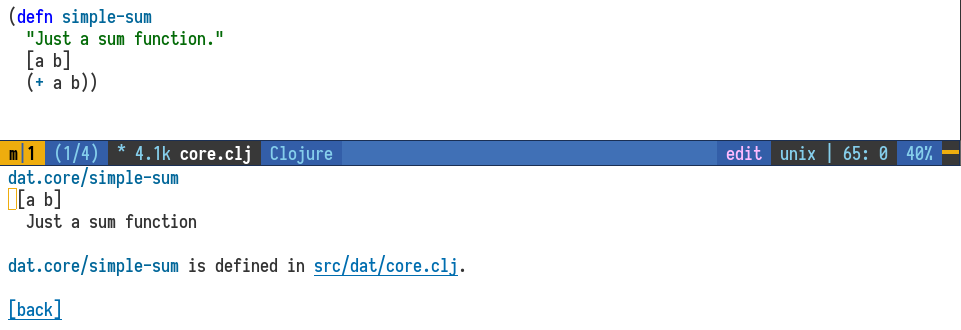
\includegraphics[width=\textwidth]{withoutspec}
% \subsection{Explanation}

Looking at documentation of function in dynamically typed language often does not
provide enough information and it is necessary to look at the source code, but
it is very time-consuming, especially when you need very small amount of
information about particular function.

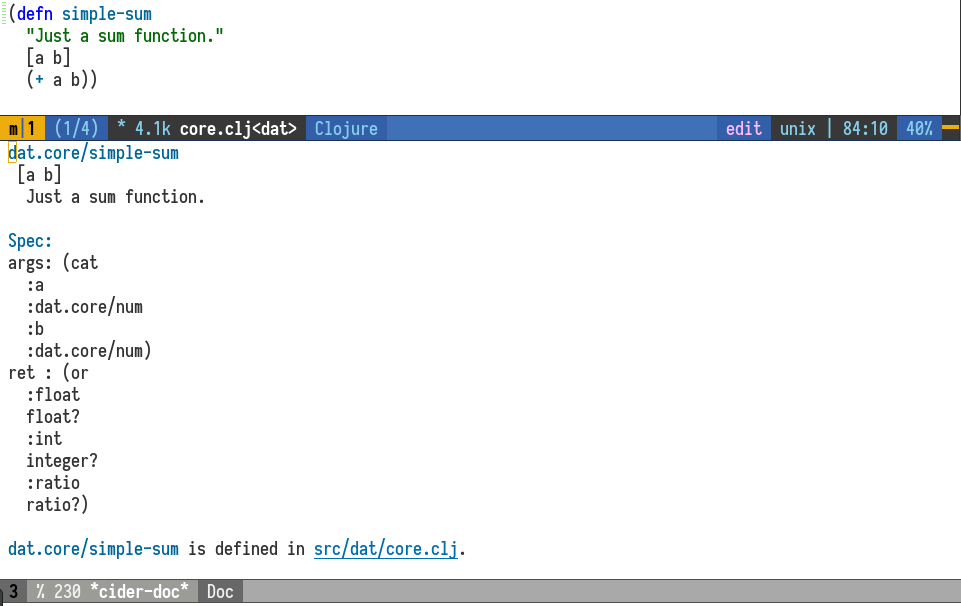
\includegraphics[width=\textwidth]{withspec}

Information about specs can be added to documentation in your IDE/repl, when
\texttt{s/fdef} macro is used. This macro defines which specs should be used for
arguments and return value, such information can be used later for sampling data
or generating documentation.

\begin{minted}{clojure}
(s/fdef simple-sum
        :args (s/cat :a ::num :b ::num)
        :ret ::num)
\end{minted}
This example provides very handy information about arguments and return value
``types'' for \texttt{simple-sum} function. Now, for developer it is not
necessary to investigate source code of the function to understand such simple
things as what parameters should be passed and what will be result of that
function. If it is not clear what mean particular spec it is easier to find its
definition and read it. Also, it is not necessary to place specs near the code,
they can be placed in separate files and namespaces as a documentation with
super cow powers.


\section{More robust software}

Let's take a look at more complex example extracted from real
commercial application. It is a part of generalized functions for REST API
testing and newcomers always has some troubles with that place. This code
simplified for thesis needs, but idea behind it is still actual.

\begin{minted}{clojure}
(def credentials
  {:admin   {:email "admin@test.io" :password "test#secret"}
   :manager {:email "manager@test.io" :password "test#secret"}
   :worker  {:email "worker@test.io" :password "test#secret"}
   :user    {:email "user@test.io" :password "test#secret"}})

(s/def ::user-type (-> credentials keys set))

(s/def ::token (s/and string?
                      #(< 6 (count %))))

(s/def ::real-token (s/and string?
                           #(< 6 (count %))
                           #(= "Token " (subs % 0 6))))

(s/def ::token-map (s/keys :req-un [::token]))

(defn get-token-for
  "Simple docstring here"
  [user-type]
  ;; somehow generate a token
  (case user-type
    :admin {:token "admin token"}
    :user {:token "user token"}
    {:token "Token default token"}))
\end{minted}


Initially, this code did not have specs and someone used to come up with
question: What user-type is? After few similar questions
\texttt{credentials} map was created. It keys is a what we call user-type and
keys is a credentials of test users, which have this particular type. Now
everyone understand that user-type is one of the following keywords:
\texttt{:admin, :manager, :worker, :user}. It is a good illustration of a better
communcation using clojure.spec, but if we already use it what else can be done
with it?

\subsection{Static analysis}
Static analysis is possible, some huge projects like CircleCI used TypedClojure
for this needs, now when spec is in active development it is more rational to
use something more suitable for it. For example, Allen Rohner develop library
for static analysis using clojure.spec. Actually it is not very natural to do
static checking in Clojure, but it can be useful in pre-commit hooks or in
continuous integration scripts. Usage is pretty simple.

\begin{minted}{clojure}
(require '[spectrum.check :as check])

(check/check 'your.namespace)
;; flow-walk exception while walking:
;; file file:/home/abcdw/repos/typed-thesis/dat/src/dat/core.clj line 139 col 1
;;  (fn* ([user-type] (case user-type :admin {:token admin token}
;;  :user {:token user token} {:token Token default token})))
\end{minted}

This check will provide error messages like classic compiler with location in
the file and problem place, but it is not very suitable for live programming and
just a good addition, which can be done for free if project already uses
clojure.spec. Also, it is not so powerful as static analysis for languages with
static type systems because specs are optional, but it probably not worse than
other gradual type systems.

\subsection{Automated test generation}
First of all, to understand how function works in general and is it works at
all, the function can be exercised if it has specs related to it and see what
values will be produced. Pretty the same as in Section \ref{sec:samplingdata}.

\begin{minted}{clojure}
(fdef get-token-for
      :args (s/cat :user-type ::user-type)
      :ret ::token-map)

(s/exercise-fn `get-token-for)
;; ([(:admin) {:token "admin token"}]
;;  [(:user) {:token "user token"}]
;;  [(:user) {:token "user token"}]
;;  [(:user) {:token "user token"}]
;;  [(:admin) {:token "admin token"}]
;;  [(:admin) {:token "admin token"}]
;;  [(:admin) {:token "admin token"}]
;;  [(:manager) {:token "Token default token"}]
;;  [(:user) {:token "user token"}]
;;  [(:user) {:token "user token"}])
\end{minted}

It works well and from samples generated above it is obvious, but how to make
sure that it will work in the future, when some changes will be added. Obvious
solutions is to write a test using generated data, but what if specs will be
changed in the future? Data will become invalid. Second solution is to generate
data on each test execution. Do it using spec.test pretty easy:

\begin{minted}{clojure}
(stest/check `get-token-for)
;; ({:spec
;;   #object[clojure.spec$fspec_impl$reify__21618 0x77325b7f
;;   "clojure.spec$fspec_impl$reify__21618@77325b7f"],
;;   :clojure.spec.test.check/ret
;;   {:result true, :num-tests 1000, :seed 1493657017408},
;;   :sym dat.core/get-token-for})
\end{minted}

To avoid flacky tests some constant seed for generators can be used, other can
be changed as well. It is like previous example, but with checking if return
value conforms the spec, in case it does not this code throws an exception. It is
already a solution, but not very good. Let's improve it. Also, we know that real
tokens is a string, which starts with ``Token '' prefix, that is why we also
change \texttt{::token-map} definition.

\begin{minted}{clojure}
(s/def ::token-map (s/keys :req-un [::real-token]))
(def test-result
  (-> (stest/check `get-token-for)
      stest/summarize-results
      with-out-str
      read-string))
;; {:spec
;;  (fspec
;;   :args
;;   (cat :user-type :dat.core/user-type)
;;   :ret
;;   :dat.core/token-map
;;   :fn
;;   nil),
;;  :sym dat.core/get-token-for,
;;  :failure
;;  {:clojure.spec/problems
;;   ({:path [:ret],
;;     :pred (contains? % :real-token),
;;     :val {:token "admin token"},
;;     :via [],
;;     :in []}),
;;   :clojure.spec.test/args (:admin),
;;   :clojure.spec.test/val {:token "admin token"},
;;   :clojure.spec/failure :check-failed}}
\end{minted}

Now, test fails and very handy hash map with results can be obtained from it.
First part of that map contains information about function specs like in
documentation example in Section \ref{sec:bettercommunication} and the second
part looks like example from Section \ref{sec:bettererrormessages}. From this
data problem place can be found easily in most cases. To create a real test it
is enough to add a simple assert in the test file.

\begin{minted}{clojure}
(when (:failure test-result) (println "test failed"))
\end{minted}

This subsection explains how to use capabilities for data generation to create
tests. Clojure is a dialect of Lisp that means that code generation is a natural
for this language and creation of such test can be even more automated using
macro, which will create tests for each speculated function in the namespace for
example.

\chapter{Lorem Ipsum}
\label{chap:ch4_abbr}
Now, for your reading pleasure, some \textsl{Lorem ipsum}, courtesy
of:
\begin{center}
\texttt{<http://www.lipsum.com/>}
\end{center}
This gives a good view of the margins --- note that the left margin
is a bit wider than the right margin to accommodate binding.

Lorem ipsum dolor sit amet, consectetur adipiscing elit. Etiam odio elit,
viverra eu tempor non, pulvinar ac nisi. Pellentesque habitant morbi
tristique senectus et netus et malesuada fames ac turpis egestas. Sed
adipiscing, dui quis viverra facilisis, quam libero adipiscing justo,
vitae dictum libero mauris ac magna. Aenean sem ligula, vulputate at
vestibulum eu, pellentesque in justo. Sed et eros mauris, sed placerat
nulla. Maecenas nulla velit, facilisis et rutrum nec, volutpat id
lorem. Duis vestibulum odio velit, id elementum tortor. Sed pellentesque
leo ac nibh iaculis at fermentum orci lobortis. Suspendisse arcu magna,
porta nec pretium non, feugiat vitae orci. Vivamus at enim arcu,
at sagittis nisl. Vestibulum at mi enim, vel malesuada justo. Class
aptent taciti sociosqu ad litora torquent per conubia nostra, per
inceptos himenaeos. Nullam sed nunc at enim posuere sagittis. Vivamus
augue turpis, mattis a blandit non, sollicitudin non nisl. Integer
vestibulum, est vitae cursus adipiscing, elit libero pretium leo,
in scelerisque augue felis volutpat nisl. Donec commodo posuere arcu,
eget feugiat dui ornare nec. Nullam eros mi, condimentum ac ultricies ac,
euismod lobortis nibh. Cras ac ligula pharetra risus elementum pharetra
vel in quam. Fusce ac augue vulputate nibh imperdiet convallis sit amet
et quam. Integer porttitor dictum fermentum.

Nullam id ante arcu. Nulla facilisi. Vestibulum sodales, mi sodales
ultricies pulvinar, orci leo dictum diam, quis imperdiet turpis lacus
ut sem. Nulla rutrum odio sit amet elit aliquam blandit gravida nunc
placerat. Aenean et neque ut leo condimentum vehicula. Fusce quis orci
vitae enim dapibus tincidunt in vel ipsum. Phasellus auctor neque ac eros
egestas sit amet ultricies erat vestibulum. Ut erat ligula, pharetra
vel hendrerit vitae, mattis ac turpis. Ut malesuada diam vitae lacus
vestibulum a tempus nisl posuere. Ut nisi sem, dictum eu laoreet sed,
commodo eget enim. Morbi vel lacus neque, tempus fringilla tellus. Nunc
id egestas felis. Nullam eu mollis neque. Ut non mauris malesuada
eros sagittis congue. Cras vitae felis ut nisl mollis semper ut quis
risus. Sed eu arcu urna, et commodo sapien. Donec vestibulum, libero
sit amet ultrices blandit, erat lorem volutpat lectus, sed feugiat leo
elit in orci. Aliquam vitae leo tellus, placerat pulvinar massa. Nulla
at sapien hendrerit diam varius vehicula.

Curabitur et orci nulla. Phasellus euismod, massa non hendrerit dictum,
dolor enim imperdiet sapien, vitae commodo lorem tellus eu quam. Duis
egestas felis velit. Sed in orci nec nulla rutrum posuere. Suspendisse
potenti. Nunc vel quam nisi. In at molestie libero. Aenean hendrerit
vestibulum orci, ut hendrerit nulla volutpat lacinia. Vestibulum sit amet
sapien vitae lectus gravida vehicula. Suspendisse ac purus sit amet est
congue auctor.

Morbi pellentesque, quam vel mattis molestie, augue purus vestibulum
lorem, nec consequat enim eros eu augue. In odio dolor, scelerisque
a lobortis porttitor, commodo ut lacus. Maecenas sit amet diam
nec tellus accumsan bibendum. Praesent in turpis velit, malesuada
commodo sapien. Nunc ornare urna enim. Sed at diam non metus porttitor
suscipit. Aliquam erat volutpat. Duis aliquet magna in mauris semper
placerat. Ut eget quam orci. Ut egestas, dolor at dapibus accumsan, leo
nibh egestas urna, ac consectetur dui odio quis eros. Nam libero dolor,
lacinia eget imperdiet non, malesuada vehicula diam. Etiam id ipsum eget
turpis consectetur tristique id at ante. Vivamus blandit nunc eu nisl
varius sed accumsan odio molestie.


% \chapter{Future Work}
\label{chap:future}

\newcommand{\BibTeX}{Bib\TeX}

\BibTeX{} can be used to handle all your bibliographic needs.  Simply add
references to the file \texttt{ref.bib} and \BibTeX\ will take care of
the rest.  An example of a \BibTeX{} book, conference paper and journal
article are given in the sample \texttt{ref.bib} file.  Many online
journals have links to \BibTeX{} citations that you can download and
incorporate into the \texttt{ref.bib} file.

The order of the fields is unimportant. \BibTeX\ will display them
in the correct order when constructing your bibliography.  Also note
that you can specify information about a reference that may not even be
included in the actual bibliography.  For example, the ISBN field is not
required by the bibliography, but you can, if you want, put the ISBN to
the \BibTeX{} entry.

% We can cite a journal article~\cite{someguy2002} and a conference
% paper~\cite{LastName1996} in the same way as a book citation.  More
% information can be found in~\cite{lam1994}.

\chapter{Conclusions}
\label{chap:conclusions}

In Chapter \ref{chap:background} introduced basic information about Clojure
language and general ideas of workflows for developers, who uses dynamically typed
languages, which supports interactive development. Most important factor
influenced decisions are stated below:

\begin{itemize}
\item Data Immutability
\item JVM/CLR/JS interopability
\item Lisp origin
\item REPL/TDD-driven development
\end{itemize}

Points above force solution not to break existing workflow and codebase, keep
feedback cycle short and be platform independent. After that was conducted from
different researches and highlighted pros and cons of static type checking with
examples. Advantages was generalized into list of three items, which was
implemented. Disadvantages was formulated to escape them. Also, existing tools
was extensively described to provide understanding why some of them chosen for
implementation. Chapter \ref{chap:implementation} explains why this points are
important and how to achieve them:

\begin{itemize}
\item Improved developer experience
\item Better communication
\item More robust software
\end{itemize}

Improved developer experience consist of three subsections: First is
destructuring and it contains descriptions how to convert shape of data using
specifications without creation of complex parser. Second is Better error
messages and it is about optional annotations can help understand location of
the problem and problem itself, moreover to get consistent experience between
platforms. Last one is sampling data explains how to use existing definitions of
data shapes to generate sample data objects, conforming those shapes.

Better communication section about understanding of existing code, interface
provided by it and documentation. It states that it is much better to generate
documentation from specs than try to maintain documentation. Specs provides many
capabilities (not only documentation generation) and tightly integrated in code
that is why they up-to-date in most cases in contrast to the documentation.

Section about robustness of software covers two main point. First is a static
analysis, which means that you can achieve most features of static world, but it
does not fit well in existing workflows. Second one is about automated software
testing, which describes generation of tests for annotated function without
significant effort.

Evaluation chapter explains trade offs, which must be accepted to get benefits
from Implementation chapter. Specs are not used for compilation and does not
affect production code because they are used in most cases only in development
environment, therefore performance neither increased, nor decreased. Size of the
code with annotations is not significantly bigger than without it. $3.3\%$ is a
good value for that.

Summing up, most of benifits is achivied for pretty sane cost. Static analysis
tools are not mature and not natural for dynamic languages. Now, it is hard to
say how this technologies and techniques will be adopted in industry, but they
looks promising.


\documentclass[a4paper,14pt]{extreport}
\usepackage[utf8]{inputenc}
\usepackage[english,russian]{babel}
% \usepackage[dvips]{graphicx}
\usepackage[pdftex]{graphicx}
\usepackage{geometry}
\geometry{left=25mm}
\geometry{right=20mm}
\geometry{top=20mm}
\geometry{bottom=20mm}
\graphicspath{{image/}}
\usepackage[usenames]{color}
\usepackage{colortbl}
\usepackage{multirow}
\usepackage{amssymb,amsfonts,amsmath,mathtext,cite,enumerate,float}
\usepackage{setspace}
\usepackage{indentfirst}
\onehalfspacing


\begin{document}
\begin{titlepage}
\begin{table}[]
    \centering
    \begin{tabular}{rcl}
    Автономная некоммерческая &
    \multirow{4}{*}{
\includegraphics[width=40mm]{image/logo.eps}}
          & Autonomous noncommercial \\
    организация высшего  & & organization of higher \\
    образования & & education \\
    «Университет Иннополис»  &
     & «Innopolis University» \\
    \hline
    \hline
    \end{tabular}
    \label{tab:my_label}
\end{table}
\vline
\vspace{20mm}

\begin{center}
\textbf{АННОТАЦИЯ \\ НА ВЫПУСКНУЮ КВАЛИФИКАЦИОННУЮ РАБОТУ  \\
ПО НАПРАВЛЕНИЮ ПОДГОТОВКИ \\ 09.03.01 --- «ИНФОРМАТИКА И ВЫЧИСЛИТЕЛЬНАЯ ТЕХНИКА»}
\end{center}
\vspace{20mm}


    \begin{tabular}{ll
|>{\columncolor[gray]{.9}}l|}
\cline{3-3}
\textbf{Тема:} &
     &
    \makebox[133mm][l]{Альтернативы статической типизации для Clojure}    \\
    &&\\
    && \\
    &&  \\
\cline{3-3}
    \end{tabular}
\vspace{5mm}


    \begin{tabular}{ll
|>{\columncolor[gray]{.9}}l|l
|>{\columncolor[gray]{.9}}l|}
\cline{3-3} \cline{5-5}
Выполнил &
     &
    \makebox[77mm][l]{Тропин Андрей Геннадьевич}   &
    &    \\
    &&&&
    \makebox[39.5mm]{\textcolor[gray]{.7}{подпись}} \\
    &&&& \\
    \cline{3-3} \cline{5-5}
    \end{tabular}
\vspace{5mm}

\vspace{\fill}

\begin{center}
Иннополис, 2017
\end{center}
\end{titlepage}


\newpage
% \noindent {\large \textbf{Содержание}} \\

\chapter*{Содержание}
\documentclass[a4paper,14pt]{report}
\usepackage[T2A]{fontenc}
\usepackage[utf8]{inputenc}
\usepackage[russian,english]{babel}
% \usepackage[dvips]{graphicx}
\usepackage[pdftex]{graphicx}
\usepackage{geometry}
\geometry{left=25mm}
\geometry{right=20mm}
\geometry{top=20mm}
\geometry{bottom=20mm}
\graphicspath{{figures/}}
\usepackage[usenames]{color}
\usepackage{colortbl}
\usepackage{multirow}
% \usepackage{setspace}
% \onehalfspacing

\usepackage{thesis}
\usepackage{minted}

\begin{document}

\pagenumbering{roman}

\include{title}

\include{abstract}
\include{ack}
\include{contents}
\include{tables}
\include{figures}

% Always make sure to tell a story in CS by using
% this order:
% 1)WHY
% 2)WHAT
% 3)HOW
\pagenumbering{arabic}
\include{chap1}
\include{chap2}
\include{chap3}
\include{chap4}
% \include{chap5}
\include{chap6}

\include{bib}

% If you have no appendices, remove the following two lines.
% If you have more appdences, add them as necessary.
\appendix
\include{apdxa}

\end{document}


% \newpage
% \noindent {\large \textbf{Введение}}
% \newline
\chapter*{Введение}

Существует два основных вида систем типизации, применяемых в современных языках
программирования: статическая и динамическая. Сторонники первого подхода
говорят, что преимущества статической проверки типов включает в себя: более
раннее обнаружение ошибок (например, предотвращает сложение переменных
строкового и целочисленного типа), дополнительную документацию и метаданные для
прогрессивного автодополнения фрагментов кода средствами интегрированной среды
разработки, а также возможность предоставлять компилятору вспомогательную
информацию, позволяющую производить оптимизации во время компиляции (например,
замена виртуальных вызовов прямыми вызовами функций).

С другой стороны, есть и сторонники динамической проверки типов, которые
считают, что языки с таким подходом имеют следующие преимущества: интерактивный
способ разработки (например, разработка на основе техник с использование REPL +
TDD, где тесты могут быть запущены без перекомпиляции всего проекта), быстрое
прототипирование (например, решения касательно типов могут быть отложены, язык
гораздо более выразителен и больше подходит для разработки систем с быстро
изменяющимися или неизвестными требования).

Статическая проверка типов - хороший инструмент, но нужно понимать, что он не
гарантирует, что программы будут безошибочными и правильными, поскольку он
обеспечивает всего лишь абстракцию во время компиляции над поведением запущенной
программной системы, это значит, что некоторые ошибки могут быть обнаружены, но
выполнение программы всё же может пойти не так. Другое, более обширное
объяснение, представленное Дэвидом Маклвером в его работе [11] более подробно
обозначает причины по которым невозможно предотвратить все ошибки во время
компиляции. Кроме того, статическая типизации заставляет разрбаотчика принимать
решения раньше, замедляет процесс компиляции и делает интерактивную разработку
практически невозможной.

В настоящее время многие люди / команды / компании заинтересованы в создании
систем оперирующих с большими объёмами данных, просто взгляните на текущие
тенденции: BigData, машинное обучение становятся все более популярными. Причина
ясна: огромные количество данных позволяет извлечь полезные знания, но для этого
нужны подходящие инструменты. Вероятно, динамичность является одним из наиболее
важных свойств языка для такого рода программных систем, поскольку большинство
данных не полностью структурировано, согласно исследовательскому отчету по
проекту Университета Беркли [10] около $95\%$. В случаях когда структура
известна заранее по прошествии нескольких шагов, люди или алгоритмы генерируют
запросы, основанные на информации и данных времени выполнения, также приобретают
динамический характер.

Динамическая проверка типов - хороший инструмент для интенсивно использующих
данные или других типов динамических систем, но важно понимать недостатки такого
подхода. Как правило приозводить рефакторинг, разрабатывать и поддерживать
системы, использующие языки с динамической типизацией сложнее, так как любое
даже небольшое изменение может в перспективе привести к краху системы, и никто
не узнает об этом, пока ошибка не возникнет позже во время выполнения. Есть
несколько техник, которые помогают справиться с проблемами такого рода, например
разработка через тестирование [1] или разработка на основе контрактов [14], но
они не решают всех проблем. Иногда удобно декларировать форму данных с помощью
спецификаций, чтобы впоследствии проверять, соответствуют ли текущие данные
формату или создавать образцы данных из таких спецификаций.

Информацию о том, когда и какой вид системы типизации лучше использовать, можно
найти в статье [13], авторы говорят, что по возможности нужно использовать
статическую типизацию и только, если необходимо - динамическую, но что, если нет
возможности выбрать систему проверки типов и необходимо использовать динамически
типизированный язык? Могут ли быть преимущества статической проверки типов
получены в таком окружении?

\chapter*{Основная часть}
% \chapter*{Заключени}



\documentclass[a4paper,14pt]{report}
\usepackage[T2A]{fontenc}
\usepackage[utf8]{inputenc}
\usepackage[russian,english]{babel}
% \usepackage[dvips]{graphicx}
\usepackage[pdftex]{graphicx}
\usepackage{geometry}
\geometry{left=25mm}
\geometry{right=20mm}
\geometry{top=20mm}
\geometry{bottom=20mm}
\graphicspath{{figures/}}
\usepackage[usenames]{color}
\usepackage{colortbl}
\usepackage{multirow}
% \usepackage{setspace}
% \onehalfspacing

\usepackage{thesis}
\usepackage{minted}

\begin{document}

\pagenumbering{roman}

\include{title}

\include{abstract}
\include{ack}
\include{contents}
\include{tables}
\include{figures}

% Always make sure to tell a story in CS by using
% this order:
% 1)WHY
% 2)WHAT
% 3)HOW
\pagenumbering{arabic}
\include{chap1}
\include{chap2}
\include{chap3}
\include{chap4}
% \include{chap5}
\include{chap6}

\include{bib}

% If you have no appendices, remove the following two lines.
% If you have more appdences, add them as necessary.
\appendix
\include{apdxa}

\end{document}

\end{document}


% If you have no appendices, remove the following two lines.
% If you have more appdences, add them as necessary.
\appendix
\chapter{Appendix}
\label{chap:appendix}
\inputminted{clojure}{./dat/src/dat/core.clj}
% \inputminted{clojure}{./dat/test/dat/core_test.clj}
% \inputminted{java}{./javacc-clojure/Clojure.jj}


% not really needed
% \inputminted{java}{./javacc-clojure/parser/ClojureParser.java}
% \inputminted{java}{./javacc-clojure/parser/ClojureParserConstants.java}


\end{document}


% \newpage
% \noindent {\large \textbf{Введение}}
% \newline
\chapter*{Введение}

Существует два основных вида систем типизации, применяемых в современных языках
программирования: статическая и динамическая. Сторонники первого подхода
говорят, что преимущества статической проверки типов включает в себя: более
раннее обнаружение ошибок (например, предотвращает сложение переменных
строкового и целочисленного типа), дополнительную документацию и метаданные для
прогрессивного автодополнения фрагментов кода средствами интегрированной среды
разработки, а также возможность предоставлять компилятору вспомогательную
информацию, позволяющую производить оптимизации во время компиляции (например,
замена виртуальных вызовов прямыми вызовами функций).

С другой стороны, есть и сторонники динамической проверки типов, которые
считают, что языки с таким подходом имеют следующие преимущества: интерактивный
способ разработки (например, разработка на основе техник с использование REPL +
TDD, где тесты могут быть запущены без перекомпиляции всего проекта), быстрое
прототипирование (например, решения касательно типов могут быть отложены, язык
гораздо более выразителен и больше подходит для разработки систем с быстро
изменяющимися или неизвестными требования).

Статическая проверка типов - хороший инструмент, но нужно понимать, что он не
гарантирует, что программы будут безошибочными и правильными, поскольку он
обеспечивает всего лишь абстракцию во время компиляции над поведением запущенной
программной системы, это значит, что некоторые ошибки могут быть обнаружены, но
выполнение программы всё же может пойти не так. Другое, более обширное
объяснение, представленное Дэвидом Маклвером в его работе [11] более подробно
обозначает причины по которым невозможно предотвратить все ошибки во время
компиляции. Кроме того, статическая типизации заставляет разрбаотчика принимать
решения раньше, замедляет процесс компиляции и делает интерактивную разработку
практически невозможной.

В настоящее время многие люди / команды / компании заинтересованы в создании
систем оперирующих с большими объёмами данных, просто взгляните на текущие
тенденции: BigData, машинное обучение становятся все более популярными. Причина
ясна: огромные количество данных позволяет извлечь полезные знания, но для этого
нужны подходящие инструменты. Вероятно, динамичность является одним из наиболее
важных свойств языка для такого рода программных систем, поскольку большинство
данных не полностью структурировано, согласно исследовательскому отчету по
проекту Университета Беркли [10] около $95\%$. В случаях когда структура
известна заранее по прошествии нескольких шагов, люди или алгоритмы генерируют
запросы, основанные на информации и данных времени выполнения, также приобретают
динамический характер.

Динамическая проверка типов - хороший инструмент для интенсивно использующих
данные или других типов динамических систем, но важно понимать недостатки такого
подхода. Как правило приозводить рефакторинг, разрабатывать и поддерживать
системы, использующие языки с динамической типизацией сложнее, так как любое
даже небольшое изменение может в перспективе привести к краху системы, и никто
не узнает об этом, пока ошибка не возникнет позже во время выполнения. Есть
несколько техник, которые помогают справиться с проблемами такого рода, например
разработка через тестирование [1] или разработка на основе контрактов [14], но
они не решают всех проблем. Иногда удобно декларировать форму данных с помощью
спецификаций, чтобы впоследствии проверять, соответствуют ли текущие данные
формату или создавать образцы данных из таких спецификаций.

Информацию о том, когда и какой вид системы типизации лучше использовать, можно
найти в статье [13], авторы говорят, что по возможности нужно использовать
статическую типизацию и только, если необходимо - динамическую, но что, если нет
возможности выбрать систему проверки типов и необходимо использовать динамически
типизированный язык? Могут ли быть преимущества статической проверки типов
получены в таком окружении?

\chapter*{Основная часть}
% \chapter*{Заключени}



\documentclass[a4paper,14pt]{report}
\usepackage[T2A]{fontenc}
\usepackage[utf8]{inputenc}
\usepackage[russian,english]{babel}
% \usepackage[dvips]{graphicx}
\usepackage[pdftex]{graphicx}
\usepackage{geometry}
\geometry{left=25mm}
\geometry{right=20mm}
\geometry{top=20mm}
\geometry{bottom=20mm}
\graphicspath{{figures/}}
\usepackage[usenames]{color}
\usepackage{colortbl}
\usepackage{multirow}
% \usepackage{setspace}
% \onehalfspacing

\usepackage{thesis}
\usepackage{minted}

\begin{document}

\pagenumbering{roman}

\begin{titlepage}
\begin{table}[]
    \centering
    \begin{tabular}{rcl}
    Автономная некоммерческая &
    \multirow{4}{*}{
\includegraphics[width=40mm]{figures/logo.eps}}
    & Autonomous noncommercial \\
    организация высшего  & & organization of higher \\
    образования & & education \\
    «Университет Иннополис»  &
     & «Innopolis University» \\
    \hline
    \hline
    \end{tabular}
    \label{tab:my_label}
\end{table}
\vline
\vspace{0mm}

\begin{center}
\textbf{
ВЫПУСКНАЯ КВАЛИФИКАЦИОННАЯ РАБОТА  \\
ПО НАПРАВЛЕНИЮ ПОДГОТОВКИ \\
09.03.01 --- «ИНФОРМАТИКА И ВЫЧИСЛИТЕЛЬНАЯ ТЕХНИКА»}
\vspace{5mm}

\textbf{GRADUATE THESIS    \\
MAJOR: "COMPUTER SCIENCE"}
\end{center}
\vspace{20mm}


    \begin{tabular}{ll
|>{\columncolor[gray]{.8}}l|}
\cline{3-3}
\textbf{Тема:} &
    \makebox[0.5mm] &
                      \makebox[135mm][l]{Альтернативы статической типизации для Clojure}    \\
    &&\\
\cline{3-3}
    \end{tabular}
\vspace{5mm}

    \begin{tabular}{ll
|>{\columncolor[gray]{.8}}l|}
\cline{3-3}
\textbf{Topic:} &
     &
       \makebox[135mm][l]{Alternatives of static type system for Clojure}    \\
    &&\\
\cline{3-3}
    \end{tabular}
\vspace{5mm}


    \begin{tabular}{ll
|>{\columncolor[gray]{.8}}l|l
|>{\columncolor[gray]{.8}}l|}
\cline{3-3} \cline{5-5}
Работу выполнил / &
    \makebox[0.5mm] &
    \makebox[64mm][l]{Тропин Андрей Геннадьевич/}  &
    &       \\
Thesis is executed by  &
    \makebox[0.5mm] &
    \makebox[64mm][l]{Tropin Andrei Gennadievich}  &
    &
    \makebox[40mm]{\textcolor[gray]{.6}{подпись / signature}}     \\
    % &&&&&
\cline{3-3} \cline{5-5}  \\
    \end{tabular}
\vspace{5mm}

    \begin{tabular}{ll
|>{\columncolor[gray]{.8}}l|l
|>{\columncolor[gray]{.8}}l|}
\cline{3-3} \cline{5-5}
Научный руководитель / &
     &
    \makebox[57mm][l]{Мануэль Маццара /}  &
    &       \\
Thesis supervisor  &
     &
    \makebox[57mm][l]{Manuel Mazzara}  &
    &
    \makebox[40mm]{\textcolor[gray]{.6}{подпись / signature}}     \\
    % &&&&&
\cline{3-3} \cline{5-5}  \\
    \end{tabular}
\vspace{\fill}

\begin{center}
Иннополис, Innopolis, 2017
\end{center}
\end{titlepage}

\addcontentsline{toc}{chapter}{Abstract}
\begin{center}
\textbf{\large Abstract}
\end{center}

This document provides information on how to workaround some drawbacks of
dynamically typed languages. Lack of documentation about function parameters
types. The need to write a lot of tests to check consistency of the project and
integration between components. Implementation hardly rely on
\textbf{clojure.spec} library.

First paragraph: state what the thesis is about, give a simple statement of aims and
methods

Second paragraph: explain the structure of the thesis and say something about the
content

Third paragraph: give a concluding statement, including a short summary of the
results

Additional information about writing abstract can be found here: \\
% https://www.th-wildau.de/fileadmin/dokumente/studiengaenge/europaeisches_management/dokumente/Dokumente_EM_Ba/Abstracts_in_English.pdf

\vspace{1cm}

% \emph{``The purpose of the abstract, which should not exceed 150 words for
% a Masters' thesis or 350 words for a Doctoral thesis, is to provide
% sufficient information to allow potential readers to decide on relevance
% of the thesis. Abstracts listed in Dissertation Abstracts International
% or Masters' Abstracts International should contain appropriate key
% words and phrases designed to assist electronic searches.''}

\hfill --- MUN School of Graduate Studies

\addcontentsline{toc}{chapter}{Acknowledgements}
\begin{center}
\textbf{\large Acknowledgements}
\end{center}

Put your acknowledgements here...

\vspace{1cm}

\emph{``Intellectual and practical assistance, advice, encouragement and
sources of monetary support should be acknowledged. It is appropriate to
acknowledge the prior publication of any material included in the thesis
either in this section or in the introductory chapter of the thesis.''}

\hfill --- MUN School of Graduate Studies

\tableofcontents

\addcontentsline{toc}{chapter}{List of Tables}
\listoftables

\addcontentsline{toc}{chapter}{List of Figures}
\listoffigures


% Always make sure to tell a story in CS by using
% this order:
% 1)WHY
% 2)WHAT
% 3)HOW
\pagenumbering{arabic}
\chapter{Introduction}
\label{chap:intro}

\section{Overview}

There are two main approaches of type checking: static and dynamic. Advocates of
first approach say that benefits of static type checking include earlier
detection of bugs and mistakes (e.g. preventing adding string to an integer),
inline documentation and additional data for advanced code competition, useful
information for compiler, which helps to make optimizations (e.g. replacing
virtual calls by direct calls, when type of the caller are known), improved
runtime efficiency (e.g. not necessary to do dynamic dispatching).

On the other hand, there are also advocates of dynamic type checking who states
that languages with such approach have following advantages: interactive dynamic
development (e.g. REPL driven development + TDD, where tests can be rerun
without recompilation of the whole project), fast prototyping (e.g. type
decisions can be postponed, language are much more expressive and more suitable
for development of systems with rapidly changing or unknown requirements).

Static type checking is a good tool, but it necessary to understand that it
doesn't guarantee programs to be bug-free and correct because it provides
compile-time abstraction over run-time behavior of the software system this
means that some errors can be caught, but execution of the program can still go
wrong. Moreover static typing force to make decisions earlier, slowdown
compilation and make interactive development nearly impossible.

Nowadays many people/teams/companies interested in making data-intensive
systems, just take a look at current trends: data-driven approaches, BigData,
machine learning becomes more and more popular. The reason is clear: huge amount
of data allows to extract useful knowledge, but we need some tools to do it.
Probably dynamism is one of the most important thing for such kind of software
systems because majority of data is not fully structured, according to research
project report of Berkeley University \ref{lymanmuch} around 95\%. In cases when
structure is known up front after few steps people or algorithms generates
queries based on run-time information and data also gets dynamic nature.

Dynamic type checking is a good tool for data-intensive or other kind of dynamic
systems, but it also necessary to understand that it has some trade-offs. It is
much harder to refactor, develop and maintain systems with such type checking
because any even small change can break the system and nobody will know it until
fault will occur later in run-time. There are some techniques, which helps to
deal with it like Test-driven development \ref{beck2003test} or Contract-driven
development \ref{meyer2007contract}, but they doesn't solve all the problems.
Sometimes it is pretty handy to define shape of the date up front to check if
current data conform the specification or to generate data samples from such
specifications.

Information about when and what type checking better to use can be found in
\cite{meijer2004static}, it states that use static typing where possible and
dynamic when needed, but what if there is no possibility to choose type checking
system and it is necessary to use dynamically typed language? Can benefits of
static type checking be achieved in such environment?


\section{Goals of the project}

One of the first tasks of a researcher is defining the scope of a study, i.e., its area (theme, field) and the amount of information to be included. Narrowing the scope of your thesis can be time-consuming. Paradoxically, the more you limit the scope, the more interesting it becomes. This is because a narrower scope lets you clarify the problem and study it at greater depth, whereas very broad research questions only allow a superficial treatment.

The research question can be formulated as one main question with (a few) more specific sub-questions or in the form of a hypothesis that will be tested.

Your research question will be your guide as your writing proceeds. If you are working independently, you are also free to modify it as you go along.

How do you know that you have drafted a research question? Most importantly, a research question is something that can be answered. If not, you have probably come up with a theme or field, not a question.

Some tips:

% I will hire someone, who will explain problems of this thesis
Use interrogative words: how, why, which (factors/situations) etc.
Some questions are closed and only invoke concrete/limited answers. Others will open up for discussions and different interpretations.
Asking “What …?” is a more closed question than asking “How?” or “In what way?”
Asking “Why” means you are investigating what causes of a phenomenon. Studying causality is methodologically demanding.
Feel free to pose partially open questions that allow discussions of the overall theme, e.g., “In what way …?”; “How can we understand [a particular phenomenon]?”
Try to condense your research question into one general question – and perhaps a few more specific sub-questions (two or three will usually suffice).

\section{Outline}
The outline gives an overview of the main points of your thesis. It clarifies the structure of your thesis and helps you find the correct focus for your work. The outline can also be used in supervision sessions, especially in the beginning. You might find that you need to restructure your thesis. Working on your outline can then be a good way of making sense of the necessary changes. A good outline shows how the different parts relate to each other, and is a useful guide for the reader.








This is the introductory chapter.  This will give you some
ideas on how to use \LaTeX~\cite{lam1994} to typeset your document.
Here is a sample quote using the \verb+\munquote+ environment:

\begin{munquote}[~\cite{lam1994}]%
\LaTeX{} is a system for typesetting documents.  Its first widely
available version, mysteriously numbered 2.09, appeared in 1985.  \LaTeX{}
is now extremely popular in the scientific and academic communities, and
it is used extensively in industry.  It has become a \emph{lingua franca}
of the scientific world; scientists send their papers electronically to
colleagues around the world in the form of \LaTeX{} input.%
\end{munquote}

The citation at the end is optional --- if you don't need it,
then use \verb+\munquote+ without any arguments:

\begin{munquote}%
Here is a quote that does not have an associated citation
after it.  You can specify the citation before or after the
quote manually.%
\end{munquote}

By default, all text is double spaced, however, quotes and footnotes
must be singled spaced.\munfootnote{This is a single spaced footnote.
SGS requires that footnotes be singled spaced and this can be done with
the \texttt{$\backslash$munfootnote} command.} The left margin is slightly
wider than the right margin.  This is to compensate for binding.

An example mathematical formulae is show in
Equation~\ref{eqn:sum}.

\begin{muneqn}{sum}
\sum_{i = 0}^{n} i^2
\end{muneqn}

A slightly more complicated equation is given in Equation~\ref{eqn:schrodinger}:
\munfootnote{Equation taken from the \textsl{Schr\"{o}dinger equation}
entry on \textsl{Wikipedia}}

\begin{muneqn}{schrodinger}
i\hbar \frac{\partial}{\partial t}\Psi(x,\,t)=
-\frac{\hbar^2}{2m}\nabla^2\Psi(x,\,t) + V(x)\Psi(x,\,t)
\end{muneqn}

\section{Cross References}
\label{sec:xrefs}

In addition to using \verb+\ref+ to refer to equations, you can also use
it (in conjunction with the \verb+\label+ command) to refer to sections
and chapters without hard coding the numbers themselves.  For example,
this is Section~\ref{sec:xrefs} of Chapter~\ref{chap:intro}.  You can
also refer to Appendix~\ref{apdx:somelabel}, Subsection~\ref{sec:nested}
below or any other place that has a \verb+\label+.  You can also use
labels to refer to a page.  For example, Chapter~\ref{chap:figtab}
starts on page~\pageref{chap:figtab}.

\section{Some Suggestions}

Here are a few recommendations:

\begin{itemize}
	\item Before using this template, make sure you check with
		your supervisor.
	\item MUN's library provides electronic access to some \LaTeX{}
		related textbooks which can be read online.  Use
		the search term \texttt{latex (computer file)} on the
		Library's web page.
	\item If you run into a problem, Google may be a helpful resource.
	\item Concentrate on content, let \LaTeX{} handle the typesetting.
	\item Don't worry about warnings related to:
	\begin{itemize}
		\item overfull \texttt{hboxes}/\texttt{boxes}
		\item underfull \texttt{hboxes}/\texttt{vboxes}
	\end{itemize}
	These can be corrected with modest rewording of your text prior
	to submission of your final copy.
\end{itemize}

\section{The \texttt{Makefile}}

You can use \texttt{make} to ``build'' your thesis on the Linux command
line\munfootnote{Linux is available on all machines running LabNet in
\textsl{The Commons} and in other computer labs on campus.} This will
automatically run the \texttt{bibtex} program to create your bibliography
and will also re-run \texttt{latex} as necessary to ensure that all
references are resolved.  A device independent file (\texttt{thesis.dvi})
will be created, by default.  If you are using this template in another
environment other than the Linux command line, then the \texttt{Makefile}
will probably not be useful to you.

\begin{itemize}
\item To make a PostScript copy of your thesis, type the following
at the command line:

\texttt{make thesis.ps}

\item To generate a PDF copy of your thesis, run:

\texttt{make thesis.pdf}

\item To generate a PDF/A-1b copy of your thesis (which should
satisfy the SGS's ethesis submission requirements):

\texttt{make ethesis.pdf}

\item To remove all the files generated by \texttt{bibtex} and
\texttt{latex}, use the command:

\texttt{make clean}

\item To remove the intermediate files, but leave the PostScript
and DVI/PDF files intact, use the command:

\texttt{make neat}
\end{itemize}

As you add or remove figures, chapters, or appendices to your thesis,
make sure you keep the \texttt{Makefile} upto date, too (see the
\texttt{FIGURES} and \texttt{FILES} macros in the \texttt{Makefile}).

\section{Changing Fonts}

Change fonts: {\Large Large},
\verb+verbatim ~@#$%^&*(){}[]+,
\textsc{Small Caps},
\textsl{slanted text},
\emph{emphasized text},
\texttt{typewriter text}.

\section{Accents and Ligatures}

Some accents:
\'{e}
\`{e}
\^{o}
\"{u}
\c{c}
\"{\i}
\'{\i}
\~{n}
\={a}
\v{a}
\u{a}

\noindent Some ligatures:
fl{\ae}ffi


\section{Some Lists}

Here is a nested enumeration:
\begin{enumerate}
	\item An enumerated list of items.
	\begin{enumerate}
		\item which can
		\item nest
		\begin{enumerate}
			\item to arbitrary
			\item levels
		\end{enumerate}
	\end{enumerate}
	\item More items
	\item in the top
	\item level list.
\end{enumerate}
Another enumeration:
\begin{enumerate}
	\item
	\begin{enumerate}
		\item Main 1 part 1
		\item Main 1 part 2
	\end{enumerate}
	\item
	\begin{enumerate}
		\item Main 2 part 1
		\item Main 2 part 2
	\end{enumerate}
\end{enumerate}

\subsection{Subsection}

\subsubsection{Subsubsection}
\label{sec:nested}
This section is referred to by Section~\ref{sec:xrefs}.

\subsubsection{Subsubsection}
\textsf{$<$Empty subsection$>$}

\chapter{Background}
\label{chap:tools}

\section{Figures}

We can include encapsulated PostScript\texttrademark\ figures
(\texttt{.eps}) in the document and refer to it using a label.
For example, MUN's logo can be seen in Figure~\ref{fig:MUN_Logo_Pantone}.
\munepsfig{MUN_Logo_Pantone}{This is MUN's logo}

Figure~\ref{fig:enrollment} shows a chart of MUN's Fall
enrollment from 2005 -- 2009.\munfootnote{From \emph{Memorial
University of Newfoundland --- Fact Book 2009}.}
\munepsfig[scale=0.50]{enrollment}{MUN Fall Enrollment 2005 -- 2009}
The figure was created using the \textsf{Calc} spreadsheet application of
the office suite \textsf{OpenOffice.org}.\munfootnote{This office suite
can be downloaded at no cost from \texttt{http://openoffice.org/}. Unlike
other commercial office suites, \textsf{OpenOffice.org} may be legally
shared with colleagues and fellow students.  There are versions for
Linux, Microsoft Windows, Mac~OS~X and Solaris.  Also, unlike commercial
offerings, \textsf{OpenOffice.org} does not require activation using
registration keys.}  This figure was reduced by 50\%.

For larger figures, we can use landscape mode to rotate the page
and display the figure using the \verb+\munlepsfig+ command, as shown
in Figure~\ref{fig:enrollment-landscape}.  The figure will be the
only thing on the page when typeset in landscape mode.
(The figure is reduced to 85\% of its original size.)
\munlepsfig[scale=0.85]{enrollment-landscape}
	{MUN Fall Enrollment 2005 -- 2009 (landscape)}

Alternatively, if we just want to rotate the figure, but not
the entire page, we can specify an \texttt{angle} attribute
in the default argument of the \verb+\munepsfig+ command.
The result is shown in Figure~\ref{fig:enrollment-rotate}.
If the figure is too large or if there isn't sufficient
text, then the figure may appear on its own page.
\munepsfig[scale=0.30,angle=90]{enrollment-rotate}
	{MUN Fall Enrollment 2005 -- 2009 (rotated)}

Note that all three of the enrollment figures are basically
the same file, but with different names --- on Linux, they are
symbolic links to the same file.  The filenames have to be different
because the reference labels need to be unique.

Figure~\ref{fig:db-deadlock} shows a Petri net created using the
\texttt{xfig} program (\texttt{http://www.xfig.org/}) which has
very good support for \LaTeX.  This figure has been
reduced to 40\% of its original size.
\munepsfig[scale=0.40]{db-deadlock}{A deadlocked Petri net}

We can also create figures of text (such as short code snippets)
using the \verb+\muntxtfig+ command, as show in Figure~\ref{fig:code}.
\begin{muntxtfig}[1.0]{code}{Hello World}{0.5\textwidth}
\begin{verbatim}
#include <stdio.h>

int main(int argc, char **argv)
{
  printf("Hello world!\n");
  exit(0);
}
\end{verbatim}
\end{muntxtfig}

\section{Tables}

We can also create tables, as seen by Table~\ref{tab:pop}.  Note that,
as required by SGS guidelines, the caption for a table appears above the
table whereas figure captions appear below the figures.  Tables and
figures can ``float'' --- they may not appear on the page on which they
are mentioned.  \LaTeX{} tries to handle figure and table placement
intelligently, but if if you have a lot of them without a reasonable
amount of surrounding textual content, the figures and tables can
accumulate towards the end of the chapter.  Generally speaking, if
there is sufficient text explaining the tables and figures or if the
tables/figures are relatively small, this may not be a problem.  However,
if you have a lot of tables or figures, it may be a good idea to put
them in an appendix and refer to them as the need arises.

\begin{muntab}{c||c|c|c||c|c|c|}{pop}{Fall Semester Enrollment}
\hline
	& \multicolumn{3}{c||}{Undergraduate}
	& \multicolumn{3}{c|}{Graduate} \\
\cline{2-7}
     & F/T & P/T & Total & F/T & P/T & Total \\
\cline{2-7}
2004 & 13,191 & 2,223 & 15,414 & 1,308 & 879 & 2,187 \\
2005 & 13,184 & 2,143 & 15,327 & 1,375 & 920 & 2,295 \\
2006 & 12,809 & 2,224 & 15,033 & 1,373 & 899 & 2,272 \\
2007 & 12,634 & 2,155 & 14,789 & 1,403 & 899 & 2,302 \\
2008 & 12,269 & 2,208 & 14,477 & 1,410 &1,005& 2,415 \\
2009 & 12,382 & 2,323 & 14,705 & 1,567 &1,106& 2,673 \\
\hline
\end{muntab}

Table~\ref{tab:degrees} shows a different table in landscape
mode.\munfootnote{This data was also taken from the \emph{Memorial
University of Newfoundland --- Fact Book 2009}.} This is useful if your
table is too wide for the page.  Tables are double-spaced by default.
To single-space a table, change the \verb+\baselinestretch+ before
beginning the table environment.  Remember to restore it after the
environment has ended.

\renewcommand{\baselinestretch}{1.0}\normalsize
\begin{munltab}{lrrrrrrrrrrrr}
	{degrees}
	{Masters Degrees Conferred by Convocation Session --- 1950 to 2009}
\cline{2-13}
				&
\multicolumn{2}{|c|}{2009}	&
\multicolumn{2}{c|}{2008}	&
\multicolumn{2}{c|}{2007}	&
\multicolumn{2}{c|}{2006}	&
\multicolumn{2}{c|}{2006}	&
\multicolumn{1}{c|}{1950--2004}	&
\multicolumn{1}{c|}{Total}	\\
\cline{2-13}
	  &
May & Oct &
May & Oct &
May & Oct &
May & Oct &
May & Oct & &  \\
Degrees \\
\hline
Master of Applied Science		&  14 &   2 &  15 &   8 &  28 &   1 &  21 &   3 &   3 &   1 &    98 &   194 \\
Master of Applied Social Psychology     &   1 &   5 &   2 &   5 &   1 &   4 &   0 &   4 &   0 &   4 &    28 &    54 \\
Master of Applied Statistics            &   0 &   0 &   3 &   1 &   0 &   0 &   1 &   0 &   0 &   0 &    19 &    24 \\
Master of Arts                          &  37 &  49 &  26 &  43 &  14 &  42 &  14 &  56 &  13 &  44 &   994 & 1,332 \\
Master of Business Administration       &  14 &  16 &  23 &   6 &  33 &  12 &  33 &  11 &  33 &   8 &   818 & 1,007 \\
Master of Education                     & 107 &  87 & 120 &  55 & 147 &  74 & 108 &  76 & 113 &  75 & 2,603 & 3,565 \\
Master of Employment Relations          &   8 &   9 &   5 &   7 &   7 &  14 &   4 &   9 &   3 &   5 &    12 &    83 \\
Master of Engineering                   &  20 &  19 &  20 &  10 &  16 &  10 &  15 &  13 &   4 &  19 &   440 &   586 \\
Master of Environmental Science         &   3 &   3 &   3 &   1 &   0 &   1 &   7 &   1 &   3 &   1 &    66 &    89 \\
Master of Marine Studies                &   2 &   0 &   0 &   1 &   0 &   2 &   2 &   2 &   1 &   2 &    26 &    38 \\
Master of Music                         &   4 &   1 &   5 &   0 &   3 &   0 &   3 &   0 &   3 &   0 &     7 &    26 \\
Master of Nursing                       &   7 &   8 &  10 &   4 &  17 &   4 &  23 &   7 &   6 &   1 &   116 &   203 \\
Master of Oil and Gas Studies           &   0 &   0 &   2 &   0 &   0 &   0 &   0 &   2 &   4 &   0 &     0 &     8 \\
Master of Philosophy                    &   5 &   4 &   2 &   1 &   5 &   2 &   5 &   3 &   2 &   0 &   112 &   141 \\
Master of Physical Education            &   0 &   2 &   3 &   0 &   5 &   4 &   3 &   0 &   4 &   4 &    84 &   109 \\
Master of Public Health                 &   0 &   8 &   0 &   0 &   0 &   0 &   0 &   0 &   0 &   0 &     0 &     8 \\
Master of Science                       &  40 &  32 &  41 &  19 &  29 &  25 &  35 &  29 &  32 &  23 & 1,653 & 1,958 \\
Master of Science (Kinesiology)         &   1 &   0 &   4 &   2 &   1 &   2 &   2 &   6 &   4 &   3 &     0 &    25 \\
Master of Science (Medicine)            &  18 &   7 &  11 &   8 &  10 &   5 &   9 &   9 &   8 &   4 &     0 &    89 \\
Master of Science (Pharmacy)            &   0 &   0 &   1 &   1 &   0 &   0 &   0 &   0 &   1 &   0 &    16 &    19 \\
Master of Social Work                   &   4 &  11 &   4 &   5 &   4 &   9 &   9 &   5 &   4 &  10 &   257 &   322 \\
Master of Women's Studies               &   2 &   0 &   2 &   0 &   1 &   1 &   2 &   3 &   2 &   0 &    20 &    33 \\
\hline
\textbf{Total Masters}                  & 287 & 263 & 302 & 177 & 321 & 212 & 296 & 239 & 243 & 204 & 7,369 & 9,913 \\
\end{munltab}
\renewcommand{\baselinestretch}{\spacing}\normalsize

\chapter{Implementation}
\label{chap:implementation}

\section{Goals}

In Chapter \ref{chap:background} was discussed three main things:
\begin{itemize}
\item Workflow and environment
\item Advantages and disadvantages of static type checking
\item Available tools and alternatives
\end{itemize}

Let's clarify what tools will be used and what we would like to achieve using
them. It necessary to keep in mind that trade offs should be sufficient, for
example feedback cycle must remain short and existing workflow should not be
broken.

First tool is clojure.spec. As mentioned in Chapter \ref{chap:background} it has
several important advantages, integrates with already existing tools and will be
part of languages in the next major release. Second tool is spectrum, which
allows to do static analysis of the code. Third is an IDE (Emacs+cider). Last
one is javacc-clojure parser, it written to assess metrics of the code for
deeper understanding of changes introduced by optional annotations.

Advantages of static type checking explained in Section
\ref{sec:statictypechecking} can be generalized and divided into three main
parts:

\begin{itemize}
\item Improved developer experience
\item Better communication
\item More robust software
\end{itemize}

On the other hand drawbacks of static type checking should be avoided when it
possible. Let's take a closer look at the points mentioned below in context of clojure.spec:

\textbf{Improved Developer Experience.} Error messages from macros are a
perennial challenge for new (and experienced) users of Clojure. Specs can be
used to conform data in macros instead of using a custom parser. And Clojure’s
macro expansion will automatically use specs, when present, to explain errors to
users. Moreover it can provide similar messages between different platforms
(jvm, clr, js). This should result in a greatly improved experience for users
when errors occur.

\textbf{Better Communication.} Clojure is a dynamic language, and thus far we have relied
on documentation or external libraries to explain the use and behavior of
functions and libraries. But documentation is difficult to produce, is
frequently not maintained, cannot be automatically checked and varies greatly in
quality. Specs are expressive and precise. Including spec in Clojure creates a
lingua franca with which we can state how our programs work and how to use them.

\textbf{More Robust Software.} Clojure has always been about simplifying the development
of robust software. In all languages, dynamic or not, tests are essential to
quality - too many critical properties are not captured by common type systems.
spec has been designed from the ground up to directly support generative testing
via test.check. When you use spec you get generative tests for free.

As an addition clojure.spec provides more power. A key advantage of
specifications over documentation is the leverage they provide. In particular,
specs can be utilized by programs in ways that docs cannot. Defining specs takes
effort, and spec aims to maximize the return you get from making that effort.
spec gives you tools for leveraging specs in documentation, validation, error
reporting, destructuring, instrumentation, test-data generation and generative
testing.

Taken together, the features of tools demonstrate the ongoing advantages of a
powerful dynamic language like Clojure for building robust software - superior
expressivity, instrumentation-enhanced REPL-driven development, sophisticated
testing and more flexible systems.

\section{Improved development experience}
This section shows how to achieve improved development experience and get
consistent error messages across different platforms.

Clojure 1.9 is in alpha state right now and there are probably no public
projects extensively using it, that is why all experiments will be conducted on
sample project. Source code provided in \ref{chap:appendix}. Let's start from
sum function example:

\subsection{Destructuring}

\begin{minted}{clojure}
(defn simple-sum
  "Just a sum function."
  [a b]
  (+ a b))
\end{minted}

Definition of the function is pretty straightforward, but in real world
functions can be slightly complex. Even in example below it is not obvious,
which types of arguments this function accepts and what it produces, but let's
clarify what arguments should be acceptable for this function by defining
\texttt{::num} spec.


\begin{minted}{clojure}
(s/def ::num (s/or :float float?
                   :int   integer?
                   :ratio ratio?))
;; => :dat.core/num
(s/def ::even-int (s/and even? integer?))
;; => :dat.core/even-int
\end{minted}

This code produces two specs with predicates composed via \texttt{s/or} and
\texttt{s/and}, which registered under \texttt{dat.core} namespace. After that
value can be validated using this spec. It is important to understand that it
provides two features: validation in the code for business logic and validation
of the code for robustness of the software product.

\begin{minted}{clojure}
(def good-numbers [0.21 1/7 42])
(def not-so-good-numbers [0.21 1/7 42 :keyword "str"])
(map #(s/valid? ::num %) not-so-good-numbers)
;; => (true true true false false)
(map #(s/valid? ::even-int %) not-so-good-numbers)
;; => (false false true false false)
\end{minted}

Nothing really special here, but let's take a look at more interesting example.
Spec can be registered, also specs can be in-place like in example below:

\begin{minted}{clojure}
(s/conform (s/coll-of ::num) good-numbers)
;; => [[:float 0.21] [:ratio 1/7] [:int 42]]
(s/conform (s/coll-of ::num) not-so-good-numbers)
;; => :clojure.spec/invalid
\end{minted}

\texttt{(s/coll-of ::num)} returns new spec as a result of function, but it is
also a great example of destructuring, it's not necessary to write additional
parser to convert your collection in more meaningful structure, it's enough to
define spec and just conform your data. It is pretty handy especially in
data-intensive applications.

\subsection{Better error messages}
\label{sec:bettererrormessages}
In the example above first conform went well, but the second produced
\texttt{:clojure.spec/invalid} keyword, but what the problem with it? Luckily,
it is easy to understand that using \texttt{s/explain} function:

\begin{minted}{clojure}
(s/explain ::even-int 0.21)
;; => "val: 0.21 fails spec: :dat.core/even-int predicate: integer?\n"

(s/explain ::even-int 5)
;; => "val: 5 fails spec: :dat.core/even-int predicate: even?\n"
\end{minted}

It looks like basic type errors in statically typed languages. It is good, but
according to reality compiler errors in many languages are very cryptic and hard
to understand. How clojure.spec would behave in more complex environment?

\begin{minted}{clojure}
(s/explain-data (s/coll-of ::num) not-so-good-numbers)

;; {:clojure.spec/problems
;;  ({:path [:float],
;;    :pred float?,
;;    :val :keyword,
;;    :via [:dat.core/num],
;;    :in [3]}
;;   {:path [:int],
;;    :pred integer?,
;;    :val :keyword,
;;    :via [:dat.core/num],
;;    :in [3]}
;;   {:path [:ratio],
;;    :pred ratio?,
;;    :val :keyword,
;;    :via [:dat.core/num],
;;    :in [3]}
;;   {:path [:float],
;;    :pred float?,
;;    :val "str",
;;    :via [:dat.core/num],
;;    :in [4]}
;;   {:path [:int],
;;    :pred integer?,
;;    :val "str",
;;    :via [:dat.core/num],
;;    :in [4]}
;;   {:path [:ratio],
;;    :pred ratio?,
;;    :val "str",
;;    :via [:dat.core/num],
;;    :in [4]})}
\end{minted}

Clojure.spec can generate error messages, but it also can generate data
structures, which contains paths of the problems. In this example it is clear
that values in \texttt{not-so-good-numbers} on position 3 and 4 are violates all
predicates in composed predicate. Resulting data structure is a list of
problems, each problem represented as a map with following keys:

\begin{itemize}
\item val - the value in the user’s input that does not match
\item spec - the spec that was being evaluated
\item at - a path (a vector of keywords) indicating the location within the spec where
the error occurred - the tags in the path correspond to any tagged part in a
spec (the alternatives in an or or alt, the parts of a cat, the keys in a map,
etc)
\item predicate - the actual predicate that was not satsified by val
\item in - the key path through a nested data val to the failing value. In this
example, the top-level value is the one that is failing so this is essentially
an empty path and is omitted.

\end{itemize}

This form of report very powerful, it not only helps developers to understand
source of problem, but also allows to deal with it programmatically, it
especially important for more complex case. In addition to it such data can be
easily visualized. Such way gives a tool for current problems and place for
future development.

\subsection{Sampling data}
\label{sec:samplingdata}
In world of programming it is very hard to give names to functions and
variables, but it also hard to come up with values for test, examples and so on,
but if we know type or even more complex predicate about data, why developers
should create sample data structures and fill them with values by hands?
Actually they do not, it is very easy to generate them from specs.

\begin{minted}{clojure}
(s/exercise ::num)
;; ([-2.0 [:float -2.0]]
;;  [-1 [:int -1]]
;;  [-2 [:int -2]]
;;  [1/2 [:ratio 1/2]]
;;  [1.0 [:float 1.0]]
;;  [1/2 [:ratio 1/2]]
;;  [8 [:int 8]]
;;  [-1 [:int -1]]
;;  [-5 [:int -5]]
;;  [7/4 [:ratio 7/4]])

(s/exercise ::even-int)
;; ([0 0]
;;  [0 0]
;;  [-4 -4]
;;  [-2 -2]
;;  [0 0]
;;  [-4 -4]
;;  [-2 -2]
;;  [0 0]
;;  [-508 -508]
;;  [1548 1548])
\end{minted}

Not only simple specs can be exercised, but more much complex. For some cases it
necessary to write specific generators, but for simple one generators provided
out of the box and works well. Moreover functions can be exercised too:

\begin{minted}{clojure}
(s/fdef simple-sum
        :args (s/cat :a ::num :b ::num)
        :ret ::num)

(s/exercise-fn `simple-sum)
;; ([(-2.0 -2.0) -4.0]
;;  [(2.0 0) 2.0]
;;  [(-2 -0.5) -2.5]
;;  [(-2 Infinity) Infinity]
;;  [(4/5 -0.625) 0.17500000000000004]
;;  [(-1 -0.5) -1.5]
;;  [(-0.5 -3/7) -0.9285714285714286]
;;  [(1/3 -1) -2/3]
;;  [(-1.0 9) 8.0]
;;  [(1.1953125 -1) 0.1953125])
\end{minted}

This example introduces new macros \texttt{s/fdef}, which will be explained
later, but in fact \texttt{s/exercise-fn} just generates data as in the previous
example, but using spec defined in \texttt{s/fdef} and passes it to function
\texttt{simple-sum}. Nothing special, but it very good basis for further steps,
like automated software testing. Information about more advanced data sampling
can be found in \cite{specific}.

\section{Better communcation}
\label{sec:bettercommunication}
Developers often use external libraries or colleague's modules or even just
their own old code, but for languages such Clojure or Python it is not obvious,
which functions accepts which values (types of values). Such information can be
placed in docstring, but the problem is that documentation is hard to maintain,
it can vary in quality, became outdated or even contradictory and it means that
it does not linked with code. Much better, when there are something built in
language like type annotations, right? Clojure.spec is enough for this needs.

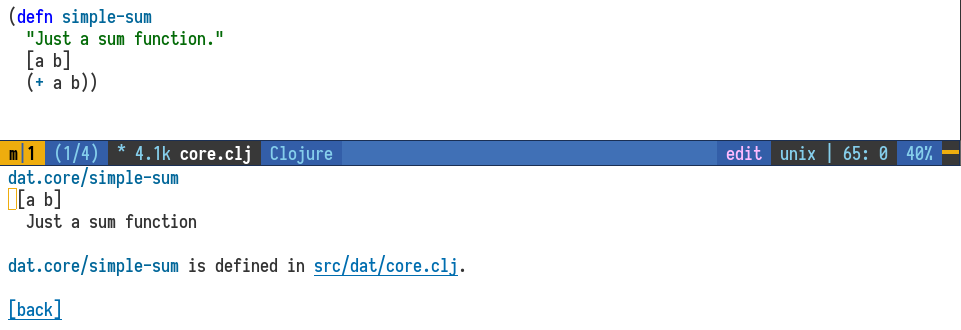
\includegraphics[width=\textwidth]{withoutspec}
% \subsection{Explanation}

Looking at documentation of function in dynamically typed language often does not
provide enough information and it is necessary to look at the source code, but
it is very time-consuming, especially when you need very small amount of
information about particular function.

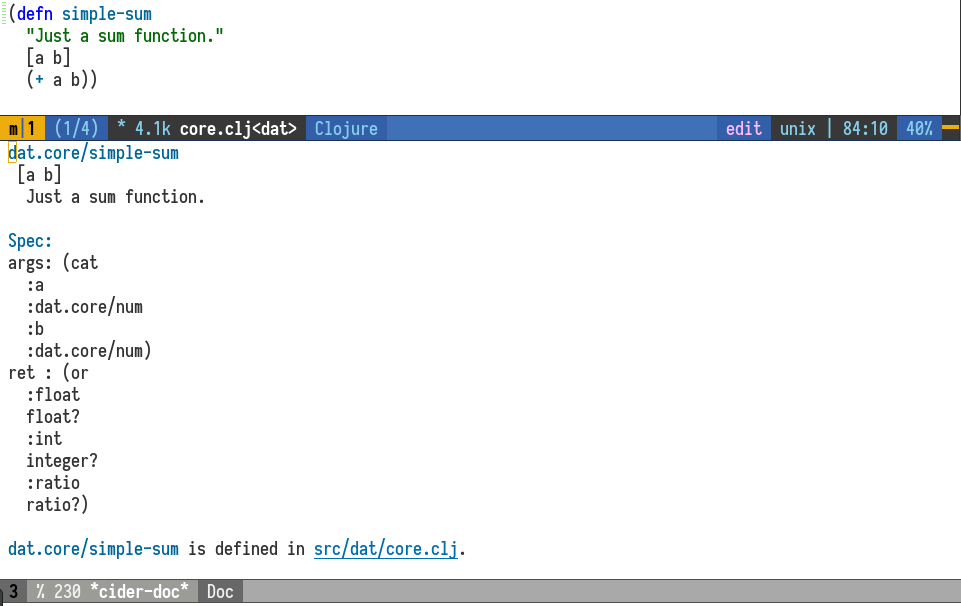
\includegraphics[width=\textwidth]{withspec}

Information about specs can be added to documentation in your IDE/repl, when
\texttt{s/fdef} macro is used. This macro defines which specs should be used for
arguments and return value, such information can be used later for sampling data
or generating documentation.

\begin{minted}{clojure}
(s/fdef simple-sum
        :args (s/cat :a ::num :b ::num)
        :ret ::num)
\end{minted}
This example provides very handy information about arguments and return value
``types'' for \texttt{simple-sum} function. Now, for developer it is not
necessary to investigate source code of the function to understand such simple
things as what parameters should be passed and what will be result of that
function. If it is not clear what mean particular spec it is easier to find its
definition and read it. Also, it is not necessary to place specs near the code,
they can be placed in separate files and namespaces as a documentation with
super cow powers.


\section{More robust software}

Let's take a look at more complex example extracted from real
commercial application. It is a part of generalized functions for REST API
testing and newcomers always has some troubles with that place. This code
simplified for thesis needs, but idea behind it is still actual.

\begin{minted}{clojure}
(def credentials
  {:admin   {:email "admin@test.io" :password "test#secret"}
   :manager {:email "manager@test.io" :password "test#secret"}
   :worker  {:email "worker@test.io" :password "test#secret"}
   :user    {:email "user@test.io" :password "test#secret"}})

(s/def ::user-type (-> credentials keys set))

(s/def ::token (s/and string?
                      #(< 6 (count %))))

(s/def ::real-token (s/and string?
                           #(< 6 (count %))
                           #(= "Token " (subs % 0 6))))

(s/def ::token-map (s/keys :req-un [::token]))

(defn get-token-for
  "Simple docstring here"
  [user-type]
  ;; somehow generate a token
  (case user-type
    :admin {:token "admin token"}
    :user {:token "user token"}
    {:token "Token default token"}))
\end{minted}


Initially, this code did not have specs and someone used to come up with
question: What user-type is? After few similar questions
\texttt{credentials} map was created. It keys is a what we call user-type and
keys is a credentials of test users, which have this particular type. Now
everyone understand that user-type is one of the following keywords:
\texttt{:admin, :manager, :worker, :user}. It is a good illustration of a better
communcation using clojure.spec, but if we already use it what else can be done
with it?

\subsection{Static analysis}
Static analysis is possible, some huge projects like CircleCI used TypedClojure
for this needs, now when spec is in active development it is more rational to
use something more suitable for it. For example, Allen Rohner develop library
for static analysis using clojure.spec. Actually it is not very natural to do
static checking in Clojure, but it can be useful in pre-commit hooks or in
continuous integration scripts. Usage is pretty simple.

\begin{minted}{clojure}
(require '[spectrum.check :as check])

(check/check 'your.namespace)
;; flow-walk exception while walking:
;; file file:/home/abcdw/repos/typed-thesis/dat/src/dat/core.clj line 139 col 1
;;  (fn* ([user-type] (case user-type :admin {:token admin token}
;;  :user {:token user token} {:token Token default token})))
\end{minted}

This check will provide error messages like classic compiler with location in
the file and problem place, but it is not very suitable for live programming and
just a good addition, which can be done for free if project already uses
clojure.spec. Also, it is not so powerful as static analysis for languages with
static type systems because specs are optional, but it probably not worse than
other gradual type systems.

\subsection{Automated test generation}
First of all, to understand how function works in general and is it works at
all, the function can be exercised if it has specs related to it and see what
values will be produced. Pretty the same as in Section \ref{sec:samplingdata}.

\begin{minted}{clojure}
(fdef get-token-for
      :args (s/cat :user-type ::user-type)
      :ret ::token-map)

(s/exercise-fn `get-token-for)
;; ([(:admin) {:token "admin token"}]
;;  [(:user) {:token "user token"}]
;;  [(:user) {:token "user token"}]
;;  [(:user) {:token "user token"}]
;;  [(:admin) {:token "admin token"}]
;;  [(:admin) {:token "admin token"}]
;;  [(:admin) {:token "admin token"}]
;;  [(:manager) {:token "Token default token"}]
;;  [(:user) {:token "user token"}]
;;  [(:user) {:token "user token"}])
\end{minted}

It works well and from samples generated above it is obvious, but how to make
sure that it will work in the future, when some changes will be added. Obvious
solutions is to write a test using generated data, but what if specs will be
changed in the future? Data will become invalid. Second solution is to generate
data on each test execution. Do it using spec.test pretty easy:

\begin{minted}{clojure}
(stest/check `get-token-for)
;; ({:spec
;;   #object[clojure.spec$fspec_impl$reify__21618 0x77325b7f
;;   "clojure.spec$fspec_impl$reify__21618@77325b7f"],
;;   :clojure.spec.test.check/ret
;;   {:result true, :num-tests 1000, :seed 1493657017408},
;;   :sym dat.core/get-token-for})
\end{minted}

To avoid flacky tests some constant seed for generators can be used, other can
be changed as well. It is like previous example, but with checking if return
value conforms the spec, in case it does not this code throws an exception. It is
already a solution, but not very good. Let's improve it. Also, we know that real
tokens is a string, which starts with ``Token '' prefix, that is why we also
change \texttt{::token-map} definition.

\begin{minted}{clojure}
(s/def ::token-map (s/keys :req-un [::real-token]))
(def test-result
  (-> (stest/check `get-token-for)
      stest/summarize-results
      with-out-str
      read-string))
;; {:spec
;;  (fspec
;;   :args
;;   (cat :user-type :dat.core/user-type)
;;   :ret
;;   :dat.core/token-map
;;   :fn
;;   nil),
;;  :sym dat.core/get-token-for,
;;  :failure
;;  {:clojure.spec/problems
;;   ({:path [:ret],
;;     :pred (contains? % :real-token),
;;     :val {:token "admin token"},
;;     :via [],
;;     :in []}),
;;   :clojure.spec.test/args (:admin),
;;   :clojure.spec.test/val {:token "admin token"},
;;   :clojure.spec/failure :check-failed}}
\end{minted}

Now, test fails and very handy hash map with results can be obtained from it.
First part of that map contains information about function specs like in
documentation example in Section \ref{sec:bettercommunication} and the second
part looks like example from Section \ref{sec:bettererrormessages}. From this
data problem place can be found easily in most cases. To create a real test it
is enough to add a simple assert in the test file.

\begin{minted}{clojure}
(when (:failure test-result) (println "test failed"))
\end{minted}

This subsection explains how to use capabilities for data generation to create
tests. Clojure is a dialect of Lisp that means that code generation is a natural
for this language and creation of such test can be even more automated using
macro, which will create tests for each speculated function in the namespace for
example.

\chapter{Lorem Ipsum}
\label{chap:ch4_abbr}
Now, for your reading pleasure, some \textsl{Lorem ipsum}, courtesy
of:
\begin{center}
\texttt{<http://www.lipsum.com/>}
\end{center}
This gives a good view of the margins --- note that the left margin
is a bit wider than the right margin to accommodate binding.

Lorem ipsum dolor sit amet, consectetur adipiscing elit. Etiam odio elit,
viverra eu tempor non, pulvinar ac nisi. Pellentesque habitant morbi
tristique senectus et netus et malesuada fames ac turpis egestas. Sed
adipiscing, dui quis viverra facilisis, quam libero adipiscing justo,
vitae dictum libero mauris ac magna. Aenean sem ligula, vulputate at
vestibulum eu, pellentesque in justo. Sed et eros mauris, sed placerat
nulla. Maecenas nulla velit, facilisis et rutrum nec, volutpat id
lorem. Duis vestibulum odio velit, id elementum tortor. Sed pellentesque
leo ac nibh iaculis at fermentum orci lobortis. Suspendisse arcu magna,
porta nec pretium non, feugiat vitae orci. Vivamus at enim arcu,
at sagittis nisl. Vestibulum at mi enim, vel malesuada justo. Class
aptent taciti sociosqu ad litora torquent per conubia nostra, per
inceptos himenaeos. Nullam sed nunc at enim posuere sagittis. Vivamus
augue turpis, mattis a blandit non, sollicitudin non nisl. Integer
vestibulum, est vitae cursus adipiscing, elit libero pretium leo,
in scelerisque augue felis volutpat nisl. Donec commodo posuere arcu,
eget feugiat dui ornare nec. Nullam eros mi, condimentum ac ultricies ac,
euismod lobortis nibh. Cras ac ligula pharetra risus elementum pharetra
vel in quam. Fusce ac augue vulputate nibh imperdiet convallis sit amet
et quam. Integer porttitor dictum fermentum.

Nullam id ante arcu. Nulla facilisi. Vestibulum sodales, mi sodales
ultricies pulvinar, orci leo dictum diam, quis imperdiet turpis lacus
ut sem. Nulla rutrum odio sit amet elit aliquam blandit gravida nunc
placerat. Aenean et neque ut leo condimentum vehicula. Fusce quis orci
vitae enim dapibus tincidunt in vel ipsum. Phasellus auctor neque ac eros
egestas sit amet ultricies erat vestibulum. Ut erat ligula, pharetra
vel hendrerit vitae, mattis ac turpis. Ut malesuada diam vitae lacus
vestibulum a tempus nisl posuere. Ut nisi sem, dictum eu laoreet sed,
commodo eget enim. Morbi vel lacus neque, tempus fringilla tellus. Nunc
id egestas felis. Nullam eu mollis neque. Ut non mauris malesuada
eros sagittis congue. Cras vitae felis ut nisl mollis semper ut quis
risus. Sed eu arcu urna, et commodo sapien. Donec vestibulum, libero
sit amet ultrices blandit, erat lorem volutpat lectus, sed feugiat leo
elit in orci. Aliquam vitae leo tellus, placerat pulvinar massa. Nulla
at sapien hendrerit diam varius vehicula.

Curabitur et orci nulla. Phasellus euismod, massa non hendrerit dictum,
dolor enim imperdiet sapien, vitae commodo lorem tellus eu quam. Duis
egestas felis velit. Sed in orci nec nulla rutrum posuere. Suspendisse
potenti. Nunc vel quam nisi. In at molestie libero. Aenean hendrerit
vestibulum orci, ut hendrerit nulla volutpat lacinia. Vestibulum sit amet
sapien vitae lectus gravida vehicula. Suspendisse ac purus sit amet est
congue auctor.

Morbi pellentesque, quam vel mattis molestie, augue purus vestibulum
lorem, nec consequat enim eros eu augue. In odio dolor, scelerisque
a lobortis porttitor, commodo ut lacus. Maecenas sit amet diam
nec tellus accumsan bibendum. Praesent in turpis velit, malesuada
commodo sapien. Nunc ornare urna enim. Sed at diam non metus porttitor
suscipit. Aliquam erat volutpat. Duis aliquet magna in mauris semper
placerat. Ut eget quam orci. Ut egestas, dolor at dapibus accumsan, leo
nibh egestas urna, ac consectetur dui odio quis eros. Nam libero dolor,
lacinia eget imperdiet non, malesuada vehicula diam. Etiam id ipsum eget
turpis consectetur tristique id at ante. Vivamus blandit nunc eu nisl
varius sed accumsan odio molestie.


% \chapter{Future Work}
\label{chap:future}

\newcommand{\BibTeX}{Bib\TeX}

\BibTeX{} can be used to handle all your bibliographic needs.  Simply add
references to the file \texttt{ref.bib} and \BibTeX\ will take care of
the rest.  An example of a \BibTeX{} book, conference paper and journal
article are given in the sample \texttt{ref.bib} file.  Many online
journals have links to \BibTeX{} citations that you can download and
incorporate into the \texttt{ref.bib} file.

The order of the fields is unimportant. \BibTeX\ will display them
in the correct order when constructing your bibliography.  Also note
that you can specify information about a reference that may not even be
included in the actual bibliography.  For example, the ISBN field is not
required by the bibliography, but you can, if you want, put the ISBN to
the \BibTeX{} entry.

% We can cite a journal article~\cite{someguy2002} and a conference
% paper~\cite{LastName1996} in the same way as a book citation.  More
% information can be found in~\cite{lam1994}.

\chapter{Conclusions}
\label{chap:conclusions}

In Chapter \ref{chap:background} introduced basic information about Clojure
language and general ideas of workflows for developers, who uses dynamically typed
languages, which supports interactive development. Most important factor
influenced decisions are stated below:

\begin{itemize}
\item Data Immutability
\item JVM/CLR/JS interopability
\item Lisp origin
\item REPL/TDD-driven development
\end{itemize}

Points above force solution not to break existing workflow and codebase, keep
feedback cycle short and be platform independent. After that was conducted from
different researches and highlighted pros and cons of static type checking with
examples. Advantages was generalized into list of three items, which was
implemented. Disadvantages was formulated to escape them. Also, existing tools
was extensively described to provide understanding why some of them chosen for
implementation. Chapter \ref{chap:implementation} explains why this points are
important and how to achieve them:

\begin{itemize}
\item Improved developer experience
\item Better communication
\item More robust software
\end{itemize}

Improved developer experience consist of three subsections: First is
destructuring and it contains descriptions how to convert shape of data using
specifications without creation of complex parser. Second is Better error
messages and it is about optional annotations can help understand location of
the problem and problem itself, moreover to get consistent experience between
platforms. Last one is sampling data explains how to use existing definitions of
data shapes to generate sample data objects, conforming those shapes.

Better communication section about understanding of existing code, interface
provided by it and documentation. It states that it is much better to generate
documentation from specs than try to maintain documentation. Specs provides many
capabilities (not only documentation generation) and tightly integrated in code
that is why they up-to-date in most cases in contrast to the documentation.

Section about robustness of software covers two main point. First is a static
analysis, which means that you can achieve most features of static world, but it
does not fit well in existing workflows. Second one is about automated software
testing, which describes generation of tests for annotated function without
significant effort.

Evaluation chapter explains trade offs, which must be accepted to get benefits
from Implementation chapter. Specs are not used for compilation and does not
affect production code because they are used in most cases only in development
environment, therefore performance neither increased, nor decreased. Size of the
code with annotations is not significantly bigger than without it. $3.3\%$ is a
good value for that.

Summing up, most of benifits is achivied for pretty sane cost. Static analysis
tools are not mature and not natural for dynamic languages. Now, it is hard to
say how this technologies and techniques will be adopted in industry, but they
looks promising.


\documentclass[a4paper,14pt]{extreport}
\usepackage[utf8]{inputenc}
\usepackage[english,russian]{babel}
% \usepackage[dvips]{graphicx}
\usepackage[pdftex]{graphicx}
\usepackage{geometry}
\geometry{left=25mm}
\geometry{right=20mm}
\geometry{top=20mm}
\geometry{bottom=20mm}
\graphicspath{{image/}}
\usepackage[usenames]{color}
\usepackage{colortbl}
\usepackage{multirow}
\usepackage{amssymb,amsfonts,amsmath,mathtext,cite,enumerate,float}
\usepackage{setspace}
\usepackage{indentfirst}
\onehalfspacing


\begin{document}
\begin{titlepage}
\begin{table}[]
    \centering
    \begin{tabular}{rcl}
    Автономная некоммерческая &
    \multirow{4}{*}{
\includegraphics[width=40mm]{image/logo.eps}}
          & Autonomous noncommercial \\
    организация высшего  & & organization of higher \\
    образования & & education \\
    «Университет Иннополис»  &
     & «Innopolis University» \\
    \hline
    \hline
    \end{tabular}
    \label{tab:my_label}
\end{table}
\vline
\vspace{20mm}

\begin{center}
\textbf{АННОТАЦИЯ \\ НА ВЫПУСКНУЮ КВАЛИФИКАЦИОННУЮ РАБОТУ  \\
ПО НАПРАВЛЕНИЮ ПОДГОТОВКИ \\ 09.03.01 --- «ИНФОРМАТИКА И ВЫЧИСЛИТЕЛЬНАЯ ТЕХНИКА»}
\end{center}
\vspace{20mm}


    \begin{tabular}{ll
|>{\columncolor[gray]{.9}}l|}
\cline{3-3}
\textbf{Тема:} &
     &
    \makebox[133mm][l]{Альтернативы статической типизации для Clojure}    \\
    &&\\
    && \\
    &&  \\
\cline{3-3}
    \end{tabular}
\vspace{5mm}


    \begin{tabular}{ll
|>{\columncolor[gray]{.9}}l|l
|>{\columncolor[gray]{.9}}l|}
\cline{3-3} \cline{5-5}
Выполнил &
     &
    \makebox[77mm][l]{Тропин Андрей Геннадьевич}   &
    &    \\
    &&&&
    \makebox[39.5mm]{\textcolor[gray]{.7}{подпись}} \\
    &&&& \\
    \cline{3-3} \cline{5-5}
    \end{tabular}
\vspace{5mm}

\vspace{\fill}

\begin{center}
Иннополис, 2017
\end{center}
\end{titlepage}


\newpage
% \noindent {\large \textbf{Содержание}} \\

\chapter*{Содержание}
\documentclass[a4paper,14pt]{report}
\usepackage[T2A]{fontenc}
\usepackage[utf8]{inputenc}
\usepackage[russian,english]{babel}
% \usepackage[dvips]{graphicx}
\usepackage[pdftex]{graphicx}
\usepackage{geometry}
\geometry{left=25mm}
\geometry{right=20mm}
\geometry{top=20mm}
\geometry{bottom=20mm}
\graphicspath{{figures/}}
\usepackage[usenames]{color}
\usepackage{colortbl}
\usepackage{multirow}
% \usepackage{setspace}
% \onehalfspacing

\usepackage{thesis}
\usepackage{minted}

\begin{document}

\pagenumbering{roman}

\include{title}

\include{abstract}
\include{ack}
\include{contents}
\include{tables}
\include{figures}

% Always make sure to tell a story in CS by using
% this order:
% 1)WHY
% 2)WHAT
% 3)HOW
\pagenumbering{arabic}
\include{chap1}
\include{chap2}
\include{chap3}
\include{chap4}
% \include{chap5}
\include{chap6}

\include{bib}

% If you have no appendices, remove the following two lines.
% If you have more appdences, add them as necessary.
\appendix
\include{apdxa}

\end{document}


% \newpage
% \noindent {\large \textbf{Введение}}
% \newline
\chapter*{Введение}

Существует два основных вида систем типизации, применяемых в современных языках
программирования: статическая и динамическая. Сторонники первого подхода
говорят, что преимущества статической проверки типов включает в себя: более
раннее обнаружение ошибок (например, предотвращает сложение переменных
строкового и целочисленного типа), дополнительную документацию и метаданные для
прогрессивного автодополнения фрагментов кода средствами интегрированной среды
разработки, а также возможность предоставлять компилятору вспомогательную
информацию, позволяющую производить оптимизации во время компиляции (например,
замена виртуальных вызовов прямыми вызовами функций).

С другой стороны, есть и сторонники динамической проверки типов, которые
считают, что языки с таким подходом имеют следующие преимущества: интерактивный
способ разработки (например, разработка на основе техник с использование REPL +
TDD, где тесты могут быть запущены без перекомпиляции всего проекта), быстрое
прототипирование (например, решения касательно типов могут быть отложены, язык
гораздо более выразителен и больше подходит для разработки систем с быстро
изменяющимися или неизвестными требования).

Статическая проверка типов - хороший инструмент, но нужно понимать, что он не
гарантирует, что программы будут безошибочными и правильными, поскольку он
обеспечивает всего лишь абстракцию во время компиляции над поведением запущенной
программной системы, это значит, что некоторые ошибки могут быть обнаружены, но
выполнение программы всё же может пойти не так. Другое, более обширное
объяснение, представленное Дэвидом Маклвером в его работе [11] более подробно
обозначает причины по которым невозможно предотвратить все ошибки во время
компиляции. Кроме того, статическая типизации заставляет разрбаотчика принимать
решения раньше, замедляет процесс компиляции и делает интерактивную разработку
практически невозможной.

В настоящее время многие люди / команды / компании заинтересованы в создании
систем оперирующих с большими объёмами данных, просто взгляните на текущие
тенденции: BigData, машинное обучение становятся все более популярными. Причина
ясна: огромные количество данных позволяет извлечь полезные знания, но для этого
нужны подходящие инструменты. Вероятно, динамичность является одним из наиболее
важных свойств языка для такого рода программных систем, поскольку большинство
данных не полностью структурировано, согласно исследовательскому отчету по
проекту Университета Беркли [10] около $95\%$. В случаях когда структура
известна заранее по прошествии нескольких шагов, люди или алгоритмы генерируют
запросы, основанные на информации и данных времени выполнения, также приобретают
динамический характер.

Динамическая проверка типов - хороший инструмент для интенсивно использующих
данные или других типов динамических систем, но важно понимать недостатки такого
подхода. Как правило приозводить рефакторинг, разрабатывать и поддерживать
системы, использующие языки с динамической типизацией сложнее, так как любое
даже небольшое изменение может в перспективе привести к краху системы, и никто
не узнает об этом, пока ошибка не возникнет позже во время выполнения. Есть
несколько техник, которые помогают справиться с проблемами такого рода, например
разработка через тестирование [1] или разработка на основе контрактов [14], но
они не решают всех проблем. Иногда удобно декларировать форму данных с помощью
спецификаций, чтобы впоследствии проверять, соответствуют ли текущие данные
формату или создавать образцы данных из таких спецификаций.

Информацию о том, когда и какой вид системы типизации лучше использовать, можно
найти в статье [13], авторы говорят, что по возможности нужно использовать
статическую типизацию и только, если необходимо - динамическую, но что, если нет
возможности выбрать систему проверки типов и необходимо использовать динамически
типизированный язык? Могут ли быть преимущества статической проверки типов
получены в таком окружении?

\chapter*{Основная часть}
% \chapter*{Заключени}



\documentclass[a4paper,14pt]{report}
\usepackage[T2A]{fontenc}
\usepackage[utf8]{inputenc}
\usepackage[russian,english]{babel}
% \usepackage[dvips]{graphicx}
\usepackage[pdftex]{graphicx}
\usepackage{geometry}
\geometry{left=25mm}
\geometry{right=20mm}
\geometry{top=20mm}
\geometry{bottom=20mm}
\graphicspath{{figures/}}
\usepackage[usenames]{color}
\usepackage{colortbl}
\usepackage{multirow}
% \usepackage{setspace}
% \onehalfspacing

\usepackage{thesis}
\usepackage{minted}

\begin{document}

\pagenumbering{roman}

\include{title}

\include{abstract}
\include{ack}
\include{contents}
\include{tables}
\include{figures}

% Always make sure to tell a story in CS by using
% this order:
% 1)WHY
% 2)WHAT
% 3)HOW
\pagenumbering{arabic}
\include{chap1}
\include{chap2}
\include{chap3}
\include{chap4}
% \include{chap5}
\include{chap6}

\include{bib}

% If you have no appendices, remove the following two lines.
% If you have more appdences, add them as necessary.
\appendix
\include{apdxa}

\end{document}

\end{document}


% If you have no appendices, remove the following two lines.
% If you have more appdences, add them as necessary.
\appendix
\chapter{Appendix}
\label{chap:appendix}
\inputminted{clojure}{./dat/src/dat/core.clj}
% \inputminted{clojure}{./dat/test/dat/core_test.clj}
% \inputminted{java}{./javacc-clojure/Clojure.jj}


% not really needed
% \inputminted{java}{./javacc-clojure/parser/ClojureParser.java}
% \inputminted{java}{./javacc-clojure/parser/ClojureParserConstants.java}


\end{document}

\end{document}
